\documentclass[12pt]{article}
\usepackage{booktabs}

\usepackage[utf8]{inputenc}
\usepackage[margin=1.2in]{geometry}
\usepackage{amsmath, amsfonts, hyperref, algorithm2e, amsthm}
\usepackage{tikz}
\usepackage{xcolor, graphicx}
\usepackage[shortlabels]{enumitem}
\usepackage{bbm}
\usetikzlibrary{snakes,arrows,shapes}

\newcommand{\E}{\mathbb{E}}
\newcommand{\Geom}{\text{Geom}}
\newcommand{\todo}[1]{\textcolor{red}{TODO: #1}}

\newtheorem{theorem}{Theorem}[section]
\newtheorem{remark}{Remark}[section]
\newtheorem{lemma}{Lemma}[section]
\theoremstyle{definition}
\newtheorem{definition}{Definition}[section]

\setlist[enumerate,1]{1.} % Level 1, 2 enumerate styles
\setlist[enumerate,2]{a.}
% \setlist[itemize,1]{$\cdot$} % Small dot

\def \title {Math 231 Project: Riding the Bus}
\def \name {Harry Sha (harry2)}
\def \date {\today}

\begin{document}

\begin{center}
    {\bf \LARGE \title}\\ \vspace{1em}
    \name\\ \vspace{1em}
    \date
\end{center}
\vspace{1em}

\begin{abstract}
    In this paper we explore the mathematics of \textit{riding the bus}, a popular card guessing game. In particular, we aim to compute and estimate the expected number of guesses and failures under different variants of the game and play strategies. We also aim to understand the distribution of guesses and failures in idealized models, and see how well these models correspond to the real world.
\end{abstract}

\vspace{3em}

\section{Introduction: riding the bus}
\paragraph{Rules and variants.}
Riding the bus is a card guessing game with simple rules. The player must make 4 correct guesses in a row and starts over from question 0 at any incorrect guess.
\begin{itemize}
    \item {\bf Question 0}: red or black? (Is the color of the next card red or black?)
    \item {\bf Question 1}: higher or lower? (Is the value of the next card higher or lower than the original card?)
    \item {\bf Question 2}: inside or outside? (Is the value of the next card in between or outside of the previous two cards?)
    \item {\bf Question 3}: suit? (What is the suit of the next card?)
\end{itemize}
When the deck runs out of cards, we reshuffle and continue. In the real world, \emph{riding the bus} is typically played as a drinking game where the cost of an incorrect guess is a sip of whatever drink you have in your hand. Therefore, this research will help determine the risks involved in playing the game, and understand the expected monetary cost of playing the game. We will study two variants of the game.

\begin{itemize}
    \item \textbf{Lenient.} In this version of the game, higher, lower, inside and outside are defined leniently in that a card is considered both higher and lower than itself.
    \item \textbf{Harsh.} In this version of the game, higher, lower, inside and outside are defined harshly in that a card is considered neither higher nor lower than itself.
\end{itemize}

In this work, we consider a generalized deck with $n$ values and $m$ suits. A deck with $n$ values and $m$ suits is modeled as $\{0,1,...,n-1\} \times \{0, 1, ...,m-1\}$. 

\paragraph{Strategies: } Define a strategy as a (possibly randomized) algorithm, $\varphi$ that takes in a history of the game so far and outputs a guess. The following are some strategies that we will analyse:
\begin{enumerate}
    \item $\varphi_{\text{drunk}}$. Select a random guess.
    \item $\varphi_{\text{greedy}}$. Selects the guess that maximizes the probability of getting the current question correctly without using memory.
    \item $\varphi_{\text{hyperthymestic}}$. Uses the same algorithm as the greedy player, except it remembers all the seen cards, and and hence knows the distribution of remaining cards in the deck.
\end{enumerate}

\paragraph{This work.} To our knowledge, no significant mathematical or statistical analyses have been conducted on riding the bus. Thus, this paper aims to answer fundamental questions related this game. At a high level, we are interested in the expected number of drinks and guesses in the game, the optimality of the greedy strategy, and the edge that can be acheived if one memorizes the cards.


\section{Infinite deck model}
\subsection{Markov chain}
In this model, we view the deck as infinitely long. The probability of drawing any card at any point in the game is $\frac{1}{mn}$. This model significantly simplifies the calculations. We can model the game played by the greedy player (note that the hyperthymestic player has no advantage in this model) as a discrete time Markov chain with the following states:

\begin{itemize}
    \item $s_{0}$, the state prior to answer question 0.
    \item $s_{1,k}$, the state prior to answering question 1, and seeing a card with value $k$.
    \item $s_{2,k}$, the state prior to answering question 2, where the absolute value of the difference of the two prior cards is $k$.
    \item $s_{3}$, the state prior to answering question 3. 
    \item $s_{4}$, the state where the game won.
\end{itemize}

Note that the strategies that we are interested in only use the value of the first card in their guess for question 1 and the absolute difference of the the value of the first two cards in the guess for question 2, so these states fully capture the game. The Markov chain for $n=4$ in the lenient variant is show in Figure \ref{fig:mc}. Of note here is that the subgraph involving the transitions from question 1 to question 2 are not a complete bipartite graph. In particular, we see that there is no transition from $s_{1, 1}$ to $s_{2, 3}$, as no value that is drawn from $\{0,1,2, 3\}$ has an absolute different of 3 with $1$.

\begin{figure}[ht]
    \begin{center}
    
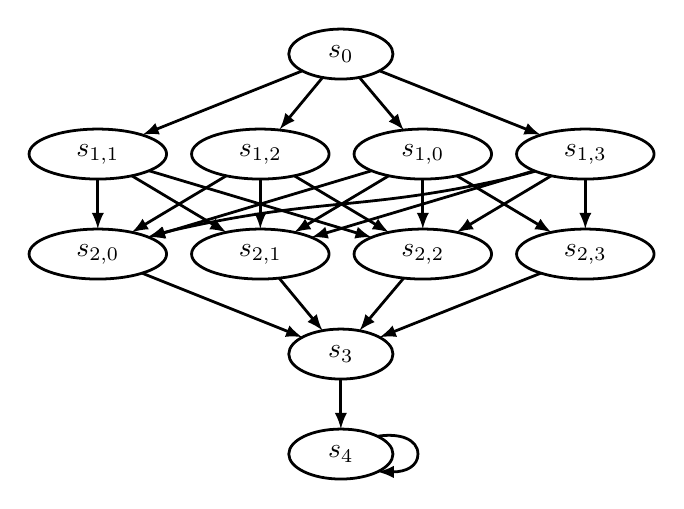
\begin{tikzpicture}[>=latex,line join=bevel,scale=0.5]
  \pgfsetlinewidth{1bp}
%%
\pgfsetcolor{black}
  % Edge: s_{0} -> s_{1, 0}
  \draw [->] (237.89bp,289.12bp) .. controls (245.33bp,280.29bp) and (254.73bp,269.13bp)  .. (269.76bp,251.31bp);
  % Edge: s_{0} -> s_{1, 1}
  \draw [->] (196.38bp,293.75bp) .. controls (168.01bp,282.41bp) and (123.88bp,264.75bp)  .. (81.706bp,247.88bp);
  % Edge: s_{0} -> s_{1, 2}
  \draw [->] (211.34bp,289.12bp) .. controls (204.13bp,280.42bp) and (195.04bp,269.45bp)  .. (180.42bp,251.8bp);
  % Edge: s_{0} -> s_{1, 3}
  \draw [->] (252.39bp,293.91bp) .. controls (281.06bp,282.5bp) and (326.04bp,264.62bp)  .. (368.27bp,247.82bp);
  % Edge: s_{1, 0} -> s_{2, 0}
  \draw [->] (246.42bp,221.91bp) .. controls (205.69bp,209.72bp) and (140.19bp,190.13bp)  .. (86.405bp,174.04bp);
  % Edge: s_{1, 0} -> s_{2, 1}
  \draw [->] (258.97bp,218.33bp) .. controls (241.73bp,208.01bp) and (218.47bp,194.1bp)  .. (190.99bp,177.65bp);
  % Edge: s_{1, 0} -> s_{2, 2}
  \draw [->] (283.5bp,215.7bp) .. controls (283.5bp,207.98bp) and (283.5bp,198.71bp)  .. (283.5bp,180.1bp);
  % Edge: s_{1, 0} -> s_{2, 3}
  \draw [->] (308.03bp,218.33bp) .. controls (325.27bp,208.01bp) and (348.53bp,194.1bp)  .. (376.01bp,177.65bp);
  % Edge: s_{1, 1} -> s_{2, 0}
  \draw [->] (49.5bp,215.7bp) .. controls (49.5bp,207.98bp) and (49.5bp,198.71bp)  .. (49.5bp,180.1bp);
  % Edge: s_{1, 1} -> s_{2, 1}
  \draw [->] (74.027bp,218.33bp) .. controls (91.265bp,208.01bp) and (114.53bp,194.1bp)  .. (142.01bp,177.65bp);
  % Edge: s_{1, 1} -> s_{2, 2}
  \draw [->] (86.578bp,221.91bp) .. controls (127.31bp,209.72bp) and (192.81bp,190.13bp)  .. (246.6bp,174.04bp);
  % Edge: s_{1, 2} -> s_{2, 0}
  \draw [->] (141.97bp,218.33bp) .. controls (124.73bp,208.01bp) and (101.47bp,194.1bp)  .. (73.995bp,177.65bp);
  % Edge: s_{1, 2} -> s_{2, 1}
  \draw [->] (166.5bp,215.7bp) .. controls (166.5bp,207.98bp) and (166.5bp,198.71bp)  .. (166.5bp,180.1bp);
  % Edge: s_{1, 2} -> s_{2, 2}
  \draw [->] (191.03bp,218.33bp) .. controls (208.27bp,208.01bp) and (231.53bp,194.1bp)  .. (259.01bp,177.65bp);
  % Edge: s_{1, 3} -> s_{2, 0}
  \draw [->] (364.49bp,221.64bp) .. controls (357.26bp,219.59bp) and (349.67bp,217.59bp)  .. (342.5bp,216.0bp) .. controls (239.35bp,193.09bp) and (210.65bp,202.91bp)  .. (107.5bp,180.0bp) .. controls (103.58bp,179.13bp) and (99.533bp,178.14bp)  .. (85.506bp,174.36bp);
  % Edge: s_{1, 3} -> s_{2, 1}
  \draw [->] (363.42bp,221.91bp) .. controls (322.69bp,209.72bp) and (257.19bp,190.13bp)  .. (203.4bp,174.04bp);
  % Edge: s_{1, 3} -> s_{2, 2}
  \draw [->] (375.97bp,218.33bp) .. controls (358.73bp,208.01bp) and (335.47bp,194.1bp)  .. (307.99bp,177.65bp);
  % Edge: s_{1, 3} -> s_{2, 3}
  \draw [->] (400.5bp,215.7bp) .. controls (400.5bp,207.98bp) and (400.5bp,198.71bp)  .. (400.5bp,180.1bp);
  % Edge: s_{2, 0} -> s_{3}
  \draw [->] (81.598bp,148.16bp) .. controls (111.47bp,136.21bp) and (155.96bp,118.41bp)  .. (196.64bp,102.14bp);
  % Edge: s_{2, 1} -> s_{3}
  \draw [->] (180.25bp,144.41bp) .. controls (187.57bp,135.57bp) and (196.72bp,124.53bp)  .. (211.25bp,106.99bp);
  % Edge: s_{2, 2} -> s_{3}
  \draw [->] (269.52bp,144.41bp) .. controls (262.06bp,135.57bp) and (252.76bp,124.53bp)  .. (237.98bp,106.99bp);
  % Edge: s_{2, 3} -> s_{3}
  \draw [->] (368.22bp,148.16bp) .. controls (338.18bp,136.21bp) and (293.43bp,118.41bp)  .. (252.52bp,102.14bp);
  % Edge: s_{3} -> s_{4}
  \draw [->] (224.5bp,71.697bp) .. controls (224.5bp,63.983bp) and (224.5bp,54.712bp)  .. (224.5bp,36.104bp);
  % Edge: s_{4} -> s_{4}
  \draw [->] (251.05bp,30.807bp) .. controls (266.08bp,33.308bp) and (280.0bp,29.039bp)  .. (280.0bp,18.0bp) .. controls (280.0bp,9.5482bp) and (271.84bp,5.0649bp)  .. (251.05bp,5.193bp);
  % Node: s_{0}
\begin{scope}
  \definecolor{strokecol}{rgb}{0.0,0.0,0.0};
  \pgfsetstrokecolor{strokecol}
  \draw (224.5bp,306.0bp) ellipse (37.5bp and 18.0bp);
  \draw (224.5bp,306.0bp) node {$s_{0}$};
\end{scope}
  % Node: s_{1, 0}
\begin{scope}
  \definecolor{strokecol}{rgb}{0.0,0.0,0.0};
  \pgfsetstrokecolor{strokecol}
  \draw (283.5bp,234.0bp) ellipse (49.5bp and 18.0bp);
  \draw (283.5bp,234.0bp) node {$s_{1, 0}$};
\end{scope}
  % Node: s_{1, 1}
\begin{scope}
  \definecolor{strokecol}{rgb}{0.0,0.0,0.0};
  \pgfsetstrokecolor{strokecol}
  \draw (49.5bp,234.0bp) ellipse (49.5bp and 18.0bp);
  \draw (49.5bp,234.0bp) node {$s_{1, 1}$};
\end{scope}
  % Node: s_{1, 2}
\begin{scope}
  \definecolor{strokecol}{rgb}{0.0,0.0,0.0};
  \pgfsetstrokecolor{strokecol}
  \draw (166.5bp,234.0bp) ellipse (49.5bp and 18.0bp);
  \draw (166.5bp,234.0bp) node {$s_{1, 2}$};
\end{scope}
  % Node: s_{1, 3}
\begin{scope}
  \definecolor{strokecol}{rgb}{0.0,0.0,0.0};
  \pgfsetstrokecolor{strokecol}
  \draw (400.5bp,234.0bp) ellipse (49.5bp and 18.0bp);
  \draw (400.5bp,234.0bp) node {$s_{1, 3}$};
\end{scope}
  % Node: s_{2, 0}
\begin{scope}
  \definecolor{strokecol}{rgb}{0.0,0.0,0.0};
  \pgfsetstrokecolor{strokecol}
  \draw (49.5bp,162.0bp) ellipse (49.5bp and 18.0bp);
  \draw (49.5bp,162.0bp) node {$s_{2, 0}$};
\end{scope}
  % Node: s_{2, 1}
\begin{scope}
  \definecolor{strokecol}{rgb}{0.0,0.0,0.0};
  \pgfsetstrokecolor{strokecol}
  \draw (166.5bp,162.0bp) ellipse (49.5bp and 18.0bp);
  \draw (166.5bp,162.0bp) node {$s_{2, 1}$};
\end{scope}
  % Node: s_{2, 2}
\begin{scope}
  \definecolor{strokecol}{rgb}{0.0,0.0,0.0};
  \pgfsetstrokecolor{strokecol}
  \draw (283.5bp,162.0bp) ellipse (49.5bp and 18.0bp);
  \draw (283.5bp,162.0bp) node {$s_{2, 2}$};
\end{scope}
  % Node: s_{2, 3}
\begin{scope}
  \definecolor{strokecol}{rgb}{0.0,0.0,0.0};
  \pgfsetstrokecolor{strokecol}
  \draw (400.5bp,162.0bp) ellipse (49.5bp and 18.0bp);
  \draw (400.5bp,162.0bp) node {$s_{2, 3}$};
\end{scope}
  % Node: s_{3}
\begin{scope}
  \definecolor{strokecol}{rgb}{0.0,0.0,0.0};
  \pgfsetstrokecolor{strokecol}
  \draw (224.5bp,90.0bp) ellipse (37.5bp and 18.0bp);
  \draw (224.5bp,90.0bp) node {$s_{3}$};
\end{scope}
  % Node: s_{4}
\begin{scope}
  \definecolor{strokecol}{rgb}{0.0,0.0,0.0};
  \pgfsetstrokecolor{strokecol}
  \draw (224.5bp,18.0bp) ellipse (37.5bp and 18.0bp);
  \draw (224.5bp,18.0bp) node {$s_{4}$};
\end{scope}
%
\end{tikzpicture}
    \end{center}
    \caption{Markov chain for $n = 4$. Note that transitions back to $s_0$ are omitted.}
    \label{fig:mc}
\end{figure}

\subsection{Transition probabilities}

Let $T(v, x, y)$ be the probability of transitioning from state $x$ to state $y$ in the $v$ variant of the game for the Markov chain described in the previous section. We'll calculate these question by question.

\paragraph{Quesion 0.} Note that regardless of the value of $n$, $m$, and $v$ we have that the probability that we guess the color of a card incorrectly is $1/2$, and thus $T(v, s_{0}, s_{0}) = 1/2$. If we guess the color correctly, it is is equally likely that the card has any of then $n$ values. Therefore for all $k \in \{0, 1,...,n-1\}$, we have $T(v, s_{0}, s_{1, k}) = \frac{1}{2n}$.

\paragraph{Quesion 1.} Having seen value $k$ after the first draw, the greedy player must then guess whether or not the next card was higher or lower. Under the lenient rules, there are $k+1$ cards `\textit{lower}' than $k$ and $n-k$ cards `\textit{higher}' than $k$. Under, the harsh rules, there are $k$ cards `\textit{lower}' than $k$ and $n-k-1$ cards `\textit{higher}' than $k$.  Let $R_1(\text{lenient}, k) = \max\{k+1, n-k\}$, and $R_1(\text{harsh}, k) = \max(k, n-k-1)$. The greedy player guesses wrong if any of $R_1(v, k)$ cards are drawn, so $T(v, s_{1, k}, s_{0,0}) = 1 - \frac{R_1(v, k)}{n}$. In the lenient version, if we guess correctly, we know that the absolute difference between the two cards is less than $R_1(\text{lenient}, k)$. In the harsh version, if we guess correctly, we know that the absolute difference between the two cards is between $1$ and $R_1(\text{harsh}, k)$. Therefore,

$$
T(\text{lenient}, s_{1,k}, s_{2, j}) = \begin{cases}
    1/n & = 0 \leq j < R_1(k)\\
    0 & \text{otherwise}
\end{cases},
$$
and
$$
T(\text{harsh}, s_{1,k}, s_{2, j}) = \begin{cases}
    1/n & 0 < j \leq R_1(k)\\
    0 & \text{otherwise}
\end{cases},
$$
for all $j, k \in \{0,1,...,n-1\}$.

\paragraph{Question 2.} If the difference between the first two cards is $k$, then under the lenient rules, there are $k+1$ numbers `\textit{inside}' them, and $\min(n-k+1, n)$ numbers `\textit{outside}' them, where we need to take the min with $n$ to account for the case where $k=0$, and under the harsh rules, there are $k-1$ `\textit{inside}' and $n-k-1$ numbers `\textit{outside}'. Let $R_2(\text{lenient}, k) = \max(k+1, \min(n-k+1, n))$, and $R_2(\text{harsh}, k) = \max(k-1, n-k-1)$, this is the number of cards that let the player move to the third question. Therefore, $T(v, s_{2, k}, s_{0,0}) = 1 - R_2(v, k) / n$, and $T(v, s_{2, k}, s_{3}) = R_2(v, k)/n$.

\paragraph{Question 3.} We get the final question correct with probability $1/m$, so $T(s_{3}, s_{4}) = 1/m$, and $T(s_{3}, s_{0}) = 1-1/m$

We are done once we get to $Q_4$, so $T(s_{4}, s_{4}) =1$. All transition probabilities that were not mentioned are have probability 0.

View $T_v$ as the transition matrix for the Markov chain, with transition probabilities defined as above, and $e_{x}$ be the vector corresponding state $x$ (1 at the index corresponding to state $x$, and 0 everywhere else).  Let $D(v, t, x) = e_{x}(T_v)^t$ be the distribution of states after $t$ time steps starting from state $x$, and let $P(v, t, x, y) = D(v, t, x)[y]$ be the probability that we are in state $y$ at time $t$ where we start from state $x$. 

\subsection{Number of drinks}
Let $N_d(v)$ be the number of drinks in a game played by the greedy player in a variant $v$ under the infinite deck model. In this section, describe the distribution of $N_d(v)$ through an analysis of the Markov chain.

\begin{theorem}
    Let 
    $$p_{\text{lenient}} = \frac{1}{2mn^3}\left(\sum_{k=0}^{n-1} \min(n, 2(n-k)) \cdot \max(k+1, \min(n-k+1, n))\right),$$
    and
    $$p_{\text{harsh}} = \frac{1}{2mn^3}\left(\sum_{k=1}^{n-1} \min(n, 2(n-k))\cdot \max(k-1, n-k-1)\right).$$ Then we have $N_d(v) \sim \Geom(p_v) - 1$
    
\end{theorem}

\begin{proof}
    The game ends when we successfully make 4 correct guesses in a row. This occurs with probability $P(v, 4, s_0, s_4)$. Therefore, the number of tries required to win the game is distributed as $\Geom(P(v, 4, s_0, s_4))$. The number of drinks is then the number of tries minus 1 (we don't drink after winning). Thus it suffices to show that $P(v, 4, s_0, s_4) = p_{v}$. We'll show the theorem for the harsh variant (the lenient variant is similar). Expanding the calculation for $P(v, 4, s_0, s_4)$, we get that

    \begin{align*}
    P(\text{harsh}, 4, s_0, s_4) &=  \frac{1}{4}P(\text{harsh}, 3, s_0, s_3)\\
    &=  \frac{1}{m}\sum_{k=1}^{n-1} T(\text{harsh}, s_{2, k}, s_3)\cdot P(\text{harsh}, 2, s_0, s_{2, k})\\
    &=  \frac{1}{mn}\sum_{k=1}^{n-1} R_2(\text{harsh}, k)\sum_{j=0}^{n-1}T(\text{harsh}, s_{1,j}, s_{2, k}) \cdot P(\text{harsh}, 1, s_0, s_{1, k})\\
    &=  \frac{1}{2mn^2}\sum_{k=1}^{n-1} R_2(\text{harsh}, k)\cdot \frac{\deg^-(s_{2k})}{n}\\
    &=  \frac{1}{2mn^3}\sum_{k=1}^{n-1} \max(k-1, n-k-1)\cdot \min(2(n-k), n)\\
    &=  p_{\text{harsh}},
    \end{align*}

    where we get the 4th equality because $T(\text{harsh}, s_{1,j}, s_{2, k})$ is $1/n$ for each $j$ that is able to transition to $s_{2, k}$ and $0$ otherwize. Thus $\sum_{j=0}^{n-1}T(\text{harsh}, s_{1,j}, s_{2, k})$ is the indegree of $s_{2, k}$ in the Markov chain divided by $n$.


\end{proof}

For a standard deck, we can plug in the $n=13$, and $m=4$, to get $p_\text{lenient} \approx 0.0793$, and $p_{\text{harsh}} \approx 0.056$. Thus we can compute $E[N_d(\text{lenient})] \approx 11.6$, and $E[N_d(\text{harsh})] \approx 16.8$. Thus we can expect to drink roughly 5 more times per game when playing the greedy strategy with the harsh rules compared to the lenient rules. The medians of the lenient and harsh variants are $\lceil -1/\log_2(1-p_\text{lenient}) \rceil - 1 = 8$, and  $\lceil -1/\log_2(1-p_\text{harsh}) \rceil - 1 = 13$ respectively and the mode of both distributions is $0$. These statistics conform pretty well to my experience playing this game as I have often been surprised by being able to get all 4 guesses on the first try, yet other times the game would go on for a long time.

An interesting implication of our theorem is that asymptotically the number of drinks depends only on the number suits in a deck and not the number of values in the deck. 

\begin{remark}
    Let $n$ and $m$ be the number of values and suits in the deck. Then $E[N_d(v)] \in \Theta(m)$. 
\end{remark}
\begin{proof}
    Note that it suffices to show that the $p_v \in \Theta(\frac{1}{m})$. To do so, we'll show that the numerator in our expression for $p_v$ is $\Theta(n^3)$. Clearly, in either variant, the numerator is $O(n^3)$ as we are summing $n$ terms that are each at most $n\cdot n$. Then it suffices to show that the numerator in the harsh variant is $\Omega(n^3)$. 

    Note that $\max(k-1, n-k-1) \geq n/2 -1$, so the numerator is at least 
    $$
    \Omega(n) \sum_{k=1}^{n-1}\min(n, 2(n-k)) \geq \Omega(n)\sum_{k=1}^{n-1}k \in \Omega(n^3)
    $$
    as required.

\end{proof}

An intuitive explanation of this result is that for large $n$, we have that picking a value from the deck approaches sampling from a uniform distribution, which does not depend on $n$, and that in order to win the game, we need to guess the final suit which requires $\Theta(m)$ tries on expectation. Table \ref{fig:ndtable} shows $E[N_d]$ for a selection of parameters.

\begin{table}[h]
\begin{center}
\begin{tabular}{@{}cccccc@{}}
\toprule
  & Variant         & $n$  & $m$  & $E[N_d]$          & Probability of winning on first try \\ \midrule
0 & lenient & 13 & 4  & 11.6& 0.079 \\
1 & lenient & 13 & 10 & 30.5& 0.031 \\
2 & lenient & 13 & 20 & 62.0& 0.015 \\
3 & lenient & 20 & 4  & 12.2& 0.075 \\
4 & lenient & 50 & 4  & 13.1& 0.070 \\
5 & harsh   & 13 & 4  & 16.8& 0.056 \\
6 & harsh   & 13 & 10 & 43.6& 0.022 \\
7 & harsh   & 13 & 20 & 88.2& 0.011 \\
8 & harsh   & 20 & 4  & 15.6& 0.060 \\
9 & harsh   & 50 & 4  & 14.4& 0.064 \\ \bottomrule
\end{tabular}
\caption{Expected number of drinks and winning probabilities for different variants and parameters of the game.}
\label{fig:ndtable}
\end{center}
\end{table}

\subsection{Number of Guesses}
Another quantity that we are interested in is the number of guesses in the game, $N_g(v)$, which can be seen as some sort of approximation to the time spent playing the game.

Figure \ref{fig:distmc} shows a visualization of the distribution of states in the Markov chain at selected time steps, and Figure \ref{fig:dist_questions} shows the probability of being at each question at each time step. We see that being in the final state is the most likely state by $t \approx 11$, and that the greedy player has won by $t \approx 20$ with over $50\%$ probability.

Table \ref{fig:ngtable} show statistics related to the distribution of failed guesses for the greedy strategy and the lenient variant based on a simulation of 100,000 games. In particular, we find that $E[N_g(\text{lenient})] \approx 27.9$. An interesting result from this simulation is that we are actually likely to answer questions 1 and 2 when we get there (79\%, and 82\% respectively), and are expected to fail on those questions only about once per game.

\begin{table}[h]
    \begin{center}
        \begin{tabular}{@{}cccccc@{}}
        \toprule
                    & fail of q0 & fail on q1 & fail on q2 & fail on q3 & $N_g$ \\ \midrule
        Probability & 0.50        & 0.79       & 0.81       & 0.25       & -                 \\
        Mean        & 6.3        & 1.3        & 1.0        & 3.0          & 27.9          \\ \bottomrule
        \end{tabular}
        \caption{Distribution of failed guesses for the greedy strategy in the lenient variant under the infinite deck model.}
        \label{fig:ngtable}
        
    \end{center}
\end{table}

\begin{figure}[h]
    \begin{center}
        \begin{minipage}{.24\textwidth}
        
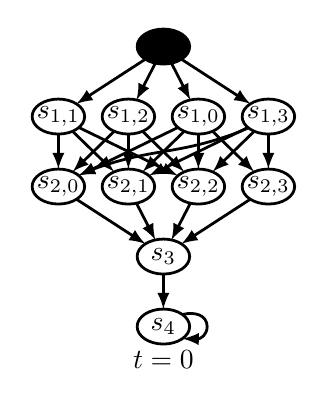
\begin{tikzpicture}[>=latex,line join=bevel,scale=0.35]
  \pgfsetlinewidth{1bp}
%%
\begin{scope}
  \definecolor{strokecol}{rgb}{0.0,0.0,0.0};
  \pgfsetstrokecolor{strokecol}
  \draw (135.0bp,16.0bp) node {$t=0$};
\end{scope}
  \pgfsetcolor{black}
  % Edge: s_{0} -> s_{1, 0}
  \draw [->] (143.35bp,320.76bp) .. controls (147.71bp,312.28bp) and (153.15bp,301.71bp)  .. (162.7bp,283.15bp);
  % Edge: s_{0} -> s_{1, 1}
  \draw [->] (116.19bp,324.81bp) .. controls (98.998bp,313.67bp) and (73.382bp,297.06bp)  .. (45.597bp,279.05bp);
  % Edge: s_{0} -> s_{1, 2}
  \draw [->] (126.65bp,320.76bp) .. controls (122.29bp,312.28bp) and (116.85bp,301.71bp)  .. (107.3bp,283.15bp);
  % Edge: s_{0} -> s_{1, 3}
  \draw [->] (153.81bp,324.81bp) .. controls (171.0bp,313.67bp) and (196.62bp,297.06bp)  .. (224.4bp,279.05bp);
  % Edge: s_{1, 0} -> s_{2, 0}
  \draw [->] (149.75bp,254.67bp) .. controls (125.4bp,242.83bp) and (85.281bp,223.33bp)  .. (48.335bp,205.37bp);
  % Edge: s_{1, 0} -> s_{2, 1}
  \draw [->] (156.43bp,250.83bp) .. controls (146.25bp,240.94bp) and (132.48bp,227.55bp)  .. (113.8bp,209.38bp);
  % Edge: s_{1, 0} -> s_{2, 2}
  \draw [->] (171.0bp,247.7bp) .. controls (171.0bp,239.98bp) and (171.0bp,230.71bp)  .. (171.0bp,212.1bp);
  % Edge: s_{1, 0} -> s_{2, 3}
  \draw [->] (185.57bp,250.83bp) .. controls (195.75bp,240.94bp) and (209.52bp,227.55bp)  .. (228.2bp,209.38bp);
  % Edge: s_{1, 1} -> s_{2, 0}
  \draw [->] (27.0bp,247.7bp) .. controls (27.0bp,239.98bp) and (27.0bp,230.71bp)  .. (27.0bp,212.1bp);
  % Edge: s_{1, 1} -> s_{2, 1}
  \draw [->] (41.57bp,250.83bp) .. controls (51.75bp,240.94bp) and (65.524bp,227.55bp)  .. (84.204bp,209.38bp);
  % Edge: s_{1, 1} -> s_{2, 2}
  \draw [->] (48.248bp,254.67bp) .. controls (72.602bp,242.83bp) and (112.72bp,223.33bp)  .. (149.67bp,205.37bp);
  % Edge: s_{1, 2} -> s_{2, 0}
  \draw [->] (84.43bp,250.83bp) .. controls (74.25bp,240.94bp) and (60.476bp,227.55bp)  .. (41.796bp,209.38bp);
  % Edge: s_{1, 2} -> s_{2, 1}
  \draw [->] (99.0bp,247.7bp) .. controls (99.0bp,239.98bp) and (99.0bp,230.71bp)  .. (99.0bp,212.1bp);
  % Edge: s_{1, 2} -> s_{2, 2}
  \draw [->] (113.57bp,250.83bp) .. controls (123.75bp,240.94bp) and (137.52bp,227.55bp)  .. (156.2bp,209.38bp);
  % Edge: s_{1, 3} -> s_{2, 0}
  \draw [->] (221.97bp,254.23bp) .. controls (217.13bp,251.98bp) and (211.95bp,249.77bp)  .. (207.0bp,248.0bp) .. controls (144.87bp,225.81bp) and (125.13bp,234.19bp)  .. (63.0bp,212.0bp) .. controls (61.145bp,211.34bp) and (59.257bp,210.61bp)  .. (48.028bp,205.77bp);
  % Edge: s_{1, 3} -> s_{2, 1}
  \draw [->] (221.75bp,254.67bp) .. controls (197.4bp,242.83bp) and (157.28bp,223.33bp)  .. (120.33bp,205.37bp);
  % Edge: s_{1, 3} -> s_{2, 2}
  \draw [->] (228.43bp,250.83bp) .. controls (218.25bp,240.94bp) and (204.48bp,227.55bp)  .. (185.8bp,209.38bp);
  % Edge: s_{1, 3} -> s_{2, 3}
  \draw [->] (243.0bp,247.7bp) .. controls (243.0bp,239.98bp) and (243.0bp,230.71bp)  .. (243.0bp,212.1bp);
  % Edge: s_{2, 0} -> s_{3}
  \draw [->] (45.812bp,180.81bp) .. controls (63.002bp,169.67bp) and (88.618bp,153.06bp)  .. (116.4bp,135.05bp);
  % Edge: s_{2, 1} -> s_{3}
  \draw [->] (107.35bp,176.76bp) .. controls (111.71bp,168.28bp) and (117.15bp,157.71bp)  .. (126.7bp,139.15bp);
  % Edge: s_{2, 2} -> s_{3}
  \draw [->] (162.65bp,176.76bp) .. controls (158.29bp,168.28bp) and (152.85bp,157.71bp)  .. (143.3bp,139.15bp);
  % Edge: s_{2, 3} -> s_{3}
  \draw [->] (224.19bp,180.81bp) .. controls (207.0bp,169.67bp) and (181.38bp,153.06bp)  .. (153.6bp,135.05bp);
  % Edge: s_{3} -> s_{4}
  \draw [->] (135.0bp,103.7bp) .. controls (135.0bp,95.983bp) and (135.0bp,86.712bp)  .. (135.0bp,68.104bp);
  % Edge: s_{4} -> s_{4}
  \draw [->] (154.9bp,62.432bp) .. controls (167.69bp,65.675bp) and (180.0bp,61.531bp)  .. (180.0bp,50.0bp) .. controls (180.0bp,41.622bp) and (173.5bp,37.143bp)  .. (154.9bp,37.568bp);
  % Node: s_{0}
\begin{scope}
  \definecolor{strokecol}{rgb}{0.0,0.0,0.0};
  \pgfsetstrokecolor{strokecol}
  \definecolor{fillcol}{rgb}{0.0,0.0,0.0};
  \pgfsetfillcolor{fillcol}
  \filldraw [opacity=1] (135.0bp,338.0bp) ellipse (27.0bp and 18.0bp);
  \draw (135.0bp,338.0bp) node {$s_{0}$};
\end{scope}
  % Node: s_{1, 0}
\begin{scope}
  \definecolor{strokecol}{rgb}{0.0,0.0,0.0};
  \pgfsetstrokecolor{strokecol}
  \definecolor{fillcol}{rgb}{1.0,1.0,1.0};
  \pgfsetfillcolor{fillcol}
  \filldraw [opacity=1] (171.0bp,266.0bp) ellipse (27.0bp and 18.0bp);
  \draw (171.0bp,266.0bp) node {$s_{1, 0}$};
\end{scope}
  % Node: s_{1, 1}
\begin{scope}
  \definecolor{strokecol}{rgb}{0.0,0.0,0.0};
  \pgfsetstrokecolor{strokecol}
  \definecolor{fillcol}{rgb}{1.0,1.0,1.0};
  \pgfsetfillcolor{fillcol}
  \filldraw [opacity=1] (27.0bp,266.0bp) ellipse (27.0bp and 18.0bp);
  \draw (27.0bp,266.0bp) node {$s_{1, 1}$};
\end{scope}
  % Node: s_{1, 2}
\begin{scope}
  \definecolor{strokecol}{rgb}{0.0,0.0,0.0};
  \pgfsetstrokecolor{strokecol}
  \definecolor{fillcol}{rgb}{1.0,1.0,1.0};
  \pgfsetfillcolor{fillcol}
  \filldraw [opacity=1] (99.0bp,266.0bp) ellipse (27.0bp and 18.0bp);
  \draw (99.0bp,266.0bp) node {$s_{1, 2}$};
\end{scope}
  % Node: s_{1, 3}
\begin{scope}
  \definecolor{strokecol}{rgb}{0.0,0.0,0.0};
  \pgfsetstrokecolor{strokecol}
  \definecolor{fillcol}{rgb}{1.0,1.0,1.0};
  \pgfsetfillcolor{fillcol}
  \filldraw [opacity=1] (243.0bp,266.0bp) ellipse (27.0bp and 18.0bp);
  \draw (243.0bp,266.0bp) node {$s_{1, 3}$};
\end{scope}
  % Node: s_{2, 0}
\begin{scope}
  \definecolor{strokecol}{rgb}{0.0,0.0,0.0};
  \pgfsetstrokecolor{strokecol}
  \definecolor{fillcol}{rgb}{1.0,1.0,1.0};
  \pgfsetfillcolor{fillcol}
  \filldraw [opacity=1] (27.0bp,194.0bp) ellipse (27.0bp and 18.0bp);
  \draw (27.0bp,194.0bp) node {$s_{2, 0}$};
\end{scope}
  % Node: s_{2, 1}
\begin{scope}
  \definecolor{strokecol}{rgb}{0.0,0.0,0.0};
  \pgfsetstrokecolor{strokecol}
  \definecolor{fillcol}{rgb}{1.0,1.0,1.0};
  \pgfsetfillcolor{fillcol}
  \filldraw [opacity=1] (99.0bp,194.0bp) ellipse (27.0bp and 18.0bp);
  \draw (99.0bp,194.0bp) node {$s_{2, 1}$};
\end{scope}
  % Node: s_{2, 2}
\begin{scope}
  \definecolor{strokecol}{rgb}{0.0,0.0,0.0};
  \pgfsetstrokecolor{strokecol}
  \definecolor{fillcol}{rgb}{1.0,1.0,1.0};
  \pgfsetfillcolor{fillcol}
  \filldraw [opacity=1] (171.0bp,194.0bp) ellipse (27.0bp and 18.0bp);
  \draw (171.0bp,194.0bp) node {$s_{2, 2}$};
\end{scope}
  % Node: s_{2, 3}
\begin{scope}
  \definecolor{strokecol}{rgb}{0.0,0.0,0.0};
  \pgfsetstrokecolor{strokecol}
  \definecolor{fillcol}{rgb}{1.0,1.0,1.0};
  \pgfsetfillcolor{fillcol}
  \filldraw [opacity=1] (243.0bp,194.0bp) ellipse (27.0bp and 18.0bp);
  \draw (243.0bp,194.0bp) node {$s_{2, 3}$};
\end{scope}
  % Node: s_{3}
\begin{scope}
  \definecolor{strokecol}{rgb}{0.0,0.0,0.0};
  \pgfsetstrokecolor{strokecol}
  \definecolor{fillcol}{rgb}{1.0,1.0,1.0};
  \pgfsetfillcolor{fillcol}
  \filldraw [opacity=1] (135.0bp,122.0bp) ellipse (27.0bp and 18.0bp);
  \draw (135.0bp,122.0bp) node {$s_{3}$};
\end{scope}
  % Node: s_{4}
\begin{scope}
  \definecolor{strokecol}{rgb}{0.0,0.0,0.0};
  \pgfsetstrokecolor{strokecol}
  \definecolor{fillcol}{rgb}{1.0,1.0,1.0};
  \pgfsetfillcolor{fillcol}
  \filldraw [opacity=1] (135.0bp,50.0bp) ellipse (27.0bp and 18.0bp);
  \draw (135.0bp,50.0bp) node {$s_{4}$};
\end{scope}
%
\end{tikzpicture}
    
        \end{minipage}
        \begin{minipage}{.24\textwidth}
        
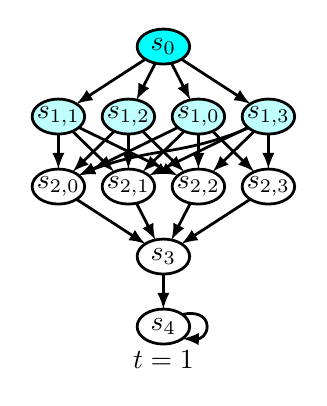
\begin{tikzpicture}[>=latex,line join=bevel,scale=0.35]
  \pgfsetlinewidth{1bp}
%%
\begin{scope}
  \definecolor{strokecol}{rgb}{0.0,0.0,0.0};
  \pgfsetstrokecolor{strokecol}
  \draw (135.0bp,16.0bp) node {$t=1$};
\end{scope}
  \pgfsetcolor{black}
  % Edge: s_{0} -> s_{1, 0}
  \draw [->] (143.35bp,320.76bp) .. controls (147.71bp,312.28bp) and (153.15bp,301.71bp)  .. (162.7bp,283.15bp);
  % Edge: s_{0} -> s_{1, 1}
  \draw [->] (116.19bp,324.81bp) .. controls (98.998bp,313.67bp) and (73.382bp,297.06bp)  .. (45.597bp,279.05bp);
  % Edge: s_{0} -> s_{1, 2}
  \draw [->] (126.65bp,320.76bp) .. controls (122.29bp,312.28bp) and (116.85bp,301.71bp)  .. (107.3bp,283.15bp);
  % Edge: s_{0} -> s_{1, 3}
  \draw [->] (153.81bp,324.81bp) .. controls (171.0bp,313.67bp) and (196.62bp,297.06bp)  .. (224.4bp,279.05bp);
  % Edge: s_{1, 0} -> s_{2, 0}
  \draw [->] (149.75bp,254.67bp) .. controls (125.4bp,242.83bp) and (85.281bp,223.33bp)  .. (48.335bp,205.37bp);
  % Edge: s_{1, 0} -> s_{2, 1}
  \draw [->] (156.43bp,250.83bp) .. controls (146.25bp,240.94bp) and (132.48bp,227.55bp)  .. (113.8bp,209.38bp);
  % Edge: s_{1, 0} -> s_{2, 2}
  \draw [->] (171.0bp,247.7bp) .. controls (171.0bp,239.98bp) and (171.0bp,230.71bp)  .. (171.0bp,212.1bp);
  % Edge: s_{1, 0} -> s_{2, 3}
  \draw [->] (185.57bp,250.83bp) .. controls (195.75bp,240.94bp) and (209.52bp,227.55bp)  .. (228.2bp,209.38bp);
  % Edge: s_{1, 1} -> s_{2, 0}
  \draw [->] (27.0bp,247.7bp) .. controls (27.0bp,239.98bp) and (27.0bp,230.71bp)  .. (27.0bp,212.1bp);
  % Edge: s_{1, 1} -> s_{2, 1}
  \draw [->] (41.57bp,250.83bp) .. controls (51.75bp,240.94bp) and (65.524bp,227.55bp)  .. (84.204bp,209.38bp);
  % Edge: s_{1, 1} -> s_{2, 2}
  \draw [->] (48.248bp,254.67bp) .. controls (72.602bp,242.83bp) and (112.72bp,223.33bp)  .. (149.67bp,205.37bp);
  % Edge: s_{1, 2} -> s_{2, 0}
  \draw [->] (84.43bp,250.83bp) .. controls (74.25bp,240.94bp) and (60.476bp,227.55bp)  .. (41.796bp,209.38bp);
  % Edge: s_{1, 2} -> s_{2, 1}
  \draw [->] (99.0bp,247.7bp) .. controls (99.0bp,239.98bp) and (99.0bp,230.71bp)  .. (99.0bp,212.1bp);
  % Edge: s_{1, 2} -> s_{2, 2}
  \draw [->] (113.57bp,250.83bp) .. controls (123.75bp,240.94bp) and (137.52bp,227.55bp)  .. (156.2bp,209.38bp);
  % Edge: s_{1, 3} -> s_{2, 0}
  \draw [->] (221.97bp,254.23bp) .. controls (217.13bp,251.98bp) and (211.95bp,249.77bp)  .. (207.0bp,248.0bp) .. controls (144.87bp,225.81bp) and (125.13bp,234.19bp)  .. (63.0bp,212.0bp) .. controls (61.145bp,211.34bp) and (59.257bp,210.61bp)  .. (48.028bp,205.77bp);
  % Edge: s_{1, 3} -> s_{2, 1}
  \draw [->] (221.75bp,254.67bp) .. controls (197.4bp,242.83bp) and (157.28bp,223.33bp)  .. (120.33bp,205.37bp);
  % Edge: s_{1, 3} -> s_{2, 2}
  \draw [->] (228.43bp,250.83bp) .. controls (218.25bp,240.94bp) and (204.48bp,227.55bp)  .. (185.8bp,209.38bp);
  % Edge: s_{1, 3} -> s_{2, 3}
  \draw [->] (243.0bp,247.7bp) .. controls (243.0bp,239.98bp) and (243.0bp,230.71bp)  .. (243.0bp,212.1bp);
  % Edge: s_{2, 0} -> s_{3}
  \draw [->] (45.812bp,180.81bp) .. controls (63.002bp,169.67bp) and (88.618bp,153.06bp)  .. (116.4bp,135.05bp);
  % Edge: s_{2, 1} -> s_{3}
  \draw [->] (107.35bp,176.76bp) .. controls (111.71bp,168.28bp) and (117.15bp,157.71bp)  .. (126.7bp,139.15bp);
  % Edge: s_{2, 2} -> s_{3}
  \draw [->] (162.65bp,176.76bp) .. controls (158.29bp,168.28bp) and (152.85bp,157.71bp)  .. (143.3bp,139.15bp);
  % Edge: s_{2, 3} -> s_{3}
  \draw [->] (224.19bp,180.81bp) .. controls (207.0bp,169.67bp) and (181.38bp,153.06bp)  .. (153.6bp,135.05bp);
  % Edge: s_{3} -> s_{4}
  \draw [->] (135.0bp,103.7bp) .. controls (135.0bp,95.983bp) and (135.0bp,86.712bp)  .. (135.0bp,68.104bp);
  % Edge: s_{4} -> s_{4}
  \draw [->] (154.9bp,62.432bp) .. controls (167.69bp,65.675bp) and (180.0bp,61.531bp)  .. (180.0bp,50.0bp) .. controls (180.0bp,41.622bp) and (173.5bp,37.143bp)  .. (154.9bp,37.568bp);
  % Node: s_{0}
\begin{scope}
  \definecolor{strokecol}{rgb}{0.0,0.0,0.0};
  \pgfsetstrokecolor{strokecol}
  \definecolor{fillcol}{rgb}{0.0,1.0,1.0};
  \pgfsetfillcolor{fillcol}
  \filldraw [opacity=1] (135.0bp,338.0bp) ellipse (27.0bp and 18.0bp);
  \draw (135.0bp,338.0bp) node {$s_{0}$};
\end{scope}
  % Node: s_{1, 0}
\begin{scope}
  \definecolor{strokecol}{rgb}{0.0,0.0,0.0};
  \pgfsetstrokecolor{strokecol}
  \definecolor{fillcol}{rgb}{0.75,1.0,1.0};
  \pgfsetfillcolor{fillcol}
  \filldraw [opacity=1] (171.0bp,266.0bp) ellipse (27.0bp and 18.0bp);
  \draw (171.0bp,266.0bp) node {$s_{1, 0}$};
\end{scope}
  % Node: s_{1, 1}
\begin{scope}
  \definecolor{strokecol}{rgb}{0.0,0.0,0.0};
  \pgfsetstrokecolor{strokecol}
  \definecolor{fillcol}{rgb}{0.75,1.0,1.0};
  \pgfsetfillcolor{fillcol}
  \filldraw [opacity=1] (27.0bp,266.0bp) ellipse (27.0bp and 18.0bp);
  \draw (27.0bp,266.0bp) node {$s_{1, 1}$};
\end{scope}
  % Node: s_{1, 2}
\begin{scope}
  \definecolor{strokecol}{rgb}{0.0,0.0,0.0};
  \pgfsetstrokecolor{strokecol}
  \definecolor{fillcol}{rgb}{0.75,1.0,1.0};
  \pgfsetfillcolor{fillcol}
  \filldraw [opacity=1] (99.0bp,266.0bp) ellipse (27.0bp and 18.0bp);
  \draw (99.0bp,266.0bp) node {$s_{1, 2}$};
\end{scope}
  % Node: s_{1, 3}
\begin{scope}
  \definecolor{strokecol}{rgb}{0.0,0.0,0.0};
  \pgfsetstrokecolor{strokecol}
  \definecolor{fillcol}{rgb}{0.75,1.0,1.0};
  \pgfsetfillcolor{fillcol}
  \filldraw [opacity=1] (243.0bp,266.0bp) ellipse (27.0bp and 18.0bp);
  \draw (243.0bp,266.0bp) node {$s_{1, 3}$};
\end{scope}
  % Node: s_{2, 0}
\begin{scope}
  \definecolor{strokecol}{rgb}{0.0,0.0,0.0};
  \pgfsetstrokecolor{strokecol}
  \definecolor{fillcol}{rgb}{1.0,1.0,1.0};
  \pgfsetfillcolor{fillcol}
  \filldraw [opacity=1] (27.0bp,194.0bp) ellipse (27.0bp and 18.0bp);
  \draw (27.0bp,194.0bp) node {$s_{2, 0}$};
\end{scope}
  % Node: s_{2, 1}
\begin{scope}
  \definecolor{strokecol}{rgb}{0.0,0.0,0.0};
  \pgfsetstrokecolor{strokecol}
  \definecolor{fillcol}{rgb}{1.0,1.0,1.0};
  \pgfsetfillcolor{fillcol}
  \filldraw [opacity=1] (99.0bp,194.0bp) ellipse (27.0bp and 18.0bp);
  \draw (99.0bp,194.0bp) node {$s_{2, 1}$};
\end{scope}
  % Node: s_{2, 2}
\begin{scope}
  \definecolor{strokecol}{rgb}{0.0,0.0,0.0};
  \pgfsetstrokecolor{strokecol}
  \definecolor{fillcol}{rgb}{1.0,1.0,1.0};
  \pgfsetfillcolor{fillcol}
  \filldraw [opacity=1] (171.0bp,194.0bp) ellipse (27.0bp and 18.0bp);
  \draw (171.0bp,194.0bp) node {$s_{2, 2}$};
\end{scope}
  % Node: s_{2, 3}
\begin{scope}
  \definecolor{strokecol}{rgb}{0.0,0.0,0.0};
  \pgfsetstrokecolor{strokecol}
  \definecolor{fillcol}{rgb}{1.0,1.0,1.0};
  \pgfsetfillcolor{fillcol}
  \filldraw [opacity=1] (243.0bp,194.0bp) ellipse (27.0bp and 18.0bp);
  \draw (243.0bp,194.0bp) node {$s_{2, 3}$};
\end{scope}
  % Node: s_{3}
\begin{scope}
  \definecolor{strokecol}{rgb}{0.0,0.0,0.0};
  \pgfsetstrokecolor{strokecol}
  \definecolor{fillcol}{rgb}{1.0,1.0,1.0};
  \pgfsetfillcolor{fillcol}
  \filldraw [opacity=1] (135.0bp,122.0bp) ellipse (27.0bp and 18.0bp);
  \draw (135.0bp,122.0bp) node {$s_{3}$};
\end{scope}
  % Node: s_{4}
\begin{scope}
  \definecolor{strokecol}{rgb}{0.0,0.0,0.0};
  \pgfsetstrokecolor{strokecol}
  \definecolor{fillcol}{rgb}{1.0,1.0,1.0};
  \pgfsetfillcolor{fillcol}
  \filldraw [opacity=1] (135.0bp,50.0bp) ellipse (27.0bp and 18.0bp);
  \draw (135.0bp,50.0bp) node {$s_{4}$};
\end{scope}
%
\end{tikzpicture}
    
        \end{minipage}
        \begin{minipage}{.24\textwidth}
        
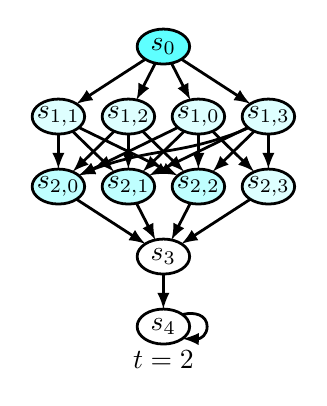
\begin{tikzpicture}[>=latex,line join=bevel,scale=0.35]
  \pgfsetlinewidth{1bp}
%%
\begin{scope}
  \definecolor{strokecol}{rgb}{0.0,0.0,0.0};
  \pgfsetstrokecolor{strokecol}
  \draw (135.0bp,16.0bp) node {$t=2$};
\end{scope}
  \pgfsetcolor{black}
  % Edge: s_{0} -> s_{1, 0}
  \draw [->] (143.35bp,320.76bp) .. controls (147.71bp,312.28bp) and (153.15bp,301.71bp)  .. (162.7bp,283.15bp);
  % Edge: s_{0} -> s_{1, 1}
  \draw [->] (116.19bp,324.81bp) .. controls (98.998bp,313.67bp) and (73.382bp,297.06bp)  .. (45.597bp,279.05bp);
  % Edge: s_{0} -> s_{1, 2}
  \draw [->] (126.65bp,320.76bp) .. controls (122.29bp,312.28bp) and (116.85bp,301.71bp)  .. (107.3bp,283.15bp);
  % Edge: s_{0} -> s_{1, 3}
  \draw [->] (153.81bp,324.81bp) .. controls (171.0bp,313.67bp) and (196.62bp,297.06bp)  .. (224.4bp,279.05bp);
  % Edge: s_{1, 0} -> s_{2, 0}
  \draw [->] (149.75bp,254.67bp) .. controls (125.4bp,242.83bp) and (85.281bp,223.33bp)  .. (48.335bp,205.37bp);
  % Edge: s_{1, 0} -> s_{2, 1}
  \draw [->] (156.43bp,250.83bp) .. controls (146.25bp,240.94bp) and (132.48bp,227.55bp)  .. (113.8bp,209.38bp);
  % Edge: s_{1, 0} -> s_{2, 2}
  \draw [->] (171.0bp,247.7bp) .. controls (171.0bp,239.98bp) and (171.0bp,230.71bp)  .. (171.0bp,212.1bp);
  % Edge: s_{1, 0} -> s_{2, 3}
  \draw [->] (185.57bp,250.83bp) .. controls (195.75bp,240.94bp) and (209.52bp,227.55bp)  .. (228.2bp,209.38bp);
  % Edge: s_{1, 1} -> s_{2, 0}
  \draw [->] (27.0bp,247.7bp) .. controls (27.0bp,239.98bp) and (27.0bp,230.71bp)  .. (27.0bp,212.1bp);
  % Edge: s_{1, 1} -> s_{2, 1}
  \draw [->] (41.57bp,250.83bp) .. controls (51.75bp,240.94bp) and (65.524bp,227.55bp)  .. (84.204bp,209.38bp);
  % Edge: s_{1, 1} -> s_{2, 2}
  \draw [->] (48.248bp,254.67bp) .. controls (72.602bp,242.83bp) and (112.72bp,223.33bp)  .. (149.67bp,205.37bp);
  % Edge: s_{1, 2} -> s_{2, 0}
  \draw [->] (84.43bp,250.83bp) .. controls (74.25bp,240.94bp) and (60.476bp,227.55bp)  .. (41.796bp,209.38bp);
  % Edge: s_{1, 2} -> s_{2, 1}
  \draw [->] (99.0bp,247.7bp) .. controls (99.0bp,239.98bp) and (99.0bp,230.71bp)  .. (99.0bp,212.1bp);
  % Edge: s_{1, 2} -> s_{2, 2}
  \draw [->] (113.57bp,250.83bp) .. controls (123.75bp,240.94bp) and (137.52bp,227.55bp)  .. (156.2bp,209.38bp);
  % Edge: s_{1, 3} -> s_{2, 0}
  \draw [->] (221.97bp,254.23bp) .. controls (217.13bp,251.98bp) and (211.95bp,249.77bp)  .. (207.0bp,248.0bp) .. controls (144.87bp,225.81bp) and (125.13bp,234.19bp)  .. (63.0bp,212.0bp) .. controls (61.145bp,211.34bp) and (59.257bp,210.61bp)  .. (48.028bp,205.77bp);
  % Edge: s_{1, 3} -> s_{2, 1}
  \draw [->] (221.75bp,254.67bp) .. controls (197.4bp,242.83bp) and (157.28bp,223.33bp)  .. (120.33bp,205.37bp);
  % Edge: s_{1, 3} -> s_{2, 2}
  \draw [->] (228.43bp,250.83bp) .. controls (218.25bp,240.94bp) and (204.48bp,227.55bp)  .. (185.8bp,209.38bp);
  % Edge: s_{1, 3} -> s_{2, 3}
  \draw [->] (243.0bp,247.7bp) .. controls (243.0bp,239.98bp) and (243.0bp,230.71bp)  .. (243.0bp,212.1bp);
  % Edge: s_{2, 0} -> s_{3}
  \draw [->] (45.812bp,180.81bp) .. controls (63.002bp,169.67bp) and (88.618bp,153.06bp)  .. (116.4bp,135.05bp);
  % Edge: s_{2, 1} -> s_{3}
  \draw [->] (107.35bp,176.76bp) .. controls (111.71bp,168.28bp) and (117.15bp,157.71bp)  .. (126.7bp,139.15bp);
  % Edge: s_{2, 2} -> s_{3}
  \draw [->] (162.65bp,176.76bp) .. controls (158.29bp,168.28bp) and (152.85bp,157.71bp)  .. (143.3bp,139.15bp);
  % Edge: s_{2, 3} -> s_{3}
  \draw [->] (224.19bp,180.81bp) .. controls (207.0bp,169.67bp) and (181.38bp,153.06bp)  .. (153.6bp,135.05bp);
  % Edge: s_{3} -> s_{4}
  \draw [->] (135.0bp,103.7bp) .. controls (135.0bp,95.983bp) and (135.0bp,86.712bp)  .. (135.0bp,68.104bp);
  % Edge: s_{4} -> s_{4}
  \draw [->] (154.9bp,62.432bp) .. controls (167.69bp,65.675bp) and (180.0bp,61.531bp)  .. (180.0bp,50.0bp) .. controls (180.0bp,41.622bp) and (173.5bp,37.143bp)  .. (154.9bp,37.568bp);
  % Node: s_{0}
\begin{scope}
  \definecolor{strokecol}{rgb}{0.0,0.0,0.0};
  \pgfsetstrokecolor{strokecol}
  \definecolor{fillcol}{rgb}{0.37,1.0,1.0};
  \pgfsetfillcolor{fillcol}
  \filldraw [opacity=1] (135.0bp,338.0bp) ellipse (27.0bp and 18.0bp);
  \draw (135.0bp,338.0bp) node {$s_{0}$};
\end{scope}
  % Node: s_{1, 0}
\begin{scope}
  \definecolor{strokecol}{rgb}{0.0,0.0,0.0};
  \pgfsetstrokecolor{strokecol}
  \definecolor{fillcol}{rgb}{0.87,1.0,1.0};
  \pgfsetfillcolor{fillcol}
  \filldraw [opacity=1] (171.0bp,266.0bp) ellipse (27.0bp and 18.0bp);
  \draw (171.0bp,266.0bp) node {$s_{1, 0}$};
\end{scope}
  % Node: s_{1, 1}
\begin{scope}
  \definecolor{strokecol}{rgb}{0.0,0.0,0.0};
  \pgfsetstrokecolor{strokecol}
  \definecolor{fillcol}{rgb}{0.87,1.0,1.0};
  \pgfsetfillcolor{fillcol}
  \filldraw [opacity=1] (27.0bp,266.0bp) ellipse (27.0bp and 18.0bp);
  \draw (27.0bp,266.0bp) node {$s_{1, 1}$};
\end{scope}
  % Node: s_{1, 2}
\begin{scope}
  \definecolor{strokecol}{rgb}{0.0,0.0,0.0};
  \pgfsetstrokecolor{strokecol}
  \definecolor{fillcol}{rgb}{0.87,1.0,1.0};
  \pgfsetfillcolor{fillcol}
  \filldraw [opacity=1] (99.0bp,266.0bp) ellipse (27.0bp and 18.0bp);
  \draw (99.0bp,266.0bp) node {$s_{1, 2}$};
\end{scope}
  % Node: s_{1, 3}
\begin{scope}
  \definecolor{strokecol}{rgb}{0.0,0.0,0.0};
  \pgfsetstrokecolor{strokecol}
  \definecolor{fillcol}{rgb}{0.87,1.0,1.0};
  \pgfsetfillcolor{fillcol}
  \filldraw [opacity=1] (243.0bp,266.0bp) ellipse (27.0bp and 18.0bp);
  \draw (243.0bp,266.0bp) node {$s_{1, 3}$};
\end{scope}
  % Node: s_{2, 0}
\begin{scope}
  \definecolor{strokecol}{rgb}{0.0,0.0,0.0};
  \pgfsetstrokecolor{strokecol}
  \definecolor{fillcol}{rgb}{0.75,1.0,1.0};
  \pgfsetfillcolor{fillcol}
  \filldraw [opacity=1] (27.0bp,194.0bp) ellipse (27.0bp and 18.0bp);
  \draw (27.0bp,194.0bp) node {$s_{2, 0}$};
\end{scope}
  % Node: s_{2, 1}
\begin{scope}
  \definecolor{strokecol}{rgb}{0.0,0.0,0.0};
  \pgfsetstrokecolor{strokecol}
  \definecolor{fillcol}{rgb}{0.75,1.0,1.0};
  \pgfsetfillcolor{fillcol}
  \filldraw [opacity=1] (99.0bp,194.0bp) ellipse (27.0bp and 18.0bp);
  \draw (99.0bp,194.0bp) node {$s_{2, 1}$};
\end{scope}
  % Node: s_{2, 2}
\begin{scope}
  \definecolor{strokecol}{rgb}{0.0,0.0,0.0};
  \pgfsetstrokecolor{strokecol}
  \definecolor{fillcol}{rgb}{0.75,1.0,1.0};
  \pgfsetfillcolor{fillcol}
  \filldraw [opacity=1] (171.0bp,194.0bp) ellipse (27.0bp and 18.0bp);
  \draw (171.0bp,194.0bp) node {$s_{2, 2}$};
\end{scope}
  % Node: s_{2, 3}
\begin{scope}
  \definecolor{strokecol}{rgb}{0.0,0.0,0.0};
  \pgfsetstrokecolor{strokecol}
  \definecolor{fillcol}{rgb}{0.87,1.0,1.0};
  \pgfsetfillcolor{fillcol}
  \filldraw [opacity=1] (243.0bp,194.0bp) ellipse (27.0bp and 18.0bp);
  \draw (243.0bp,194.0bp) node {$s_{2, 3}$};
\end{scope}
  % Node: s_{3}
\begin{scope}
  \definecolor{strokecol}{rgb}{0.0,0.0,0.0};
  \pgfsetstrokecolor{strokecol}
  \definecolor{fillcol}{rgb}{1.0,1.0,1.0};
  \pgfsetfillcolor{fillcol}
  \filldraw [opacity=1] (135.0bp,122.0bp) ellipse (27.0bp and 18.0bp);
  \draw (135.0bp,122.0bp) node {$s_{3}$};
\end{scope}
  % Node: s_{4}
\begin{scope}
  \definecolor{strokecol}{rgb}{0.0,0.0,0.0};
  \pgfsetstrokecolor{strokecol}
  \definecolor{fillcol}{rgb}{1.0,1.0,1.0};
  \pgfsetfillcolor{fillcol}
  \filldraw [opacity=1] (135.0bp,50.0bp) ellipse (27.0bp and 18.0bp);
  \draw (135.0bp,50.0bp) node {$s_{4}$};
\end{scope}
%
\end{tikzpicture}
    
        \end{minipage}
        \begin{minipage}{.24\textwidth}
        
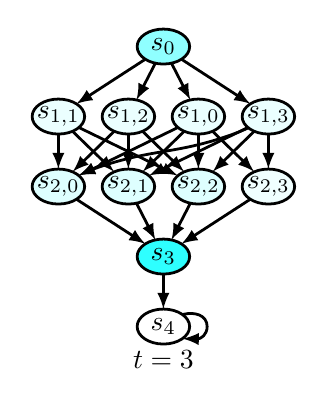
\begin{tikzpicture}[>=latex,line join=bevel,scale=0.35]
  \pgfsetlinewidth{1bp}
%%
\begin{scope}
  \definecolor{strokecol}{rgb}{0.0,0.0,0.0};
  \pgfsetstrokecolor{strokecol}
  \draw (135.0bp,16.0bp) node {$t=3$};
\end{scope}
  \pgfsetcolor{black}
  % Edge: s_{0} -> s_{1, 0}
  \draw [->] (143.35bp,320.76bp) .. controls (147.71bp,312.28bp) and (153.15bp,301.71bp)  .. (162.7bp,283.15bp);
  % Edge: s_{0} -> s_{1, 1}
  \draw [->] (116.19bp,324.81bp) .. controls (98.998bp,313.67bp) and (73.382bp,297.06bp)  .. (45.597bp,279.05bp);
  % Edge: s_{0} -> s_{1, 2}
  \draw [->] (126.65bp,320.76bp) .. controls (122.29bp,312.28bp) and (116.85bp,301.71bp)  .. (107.3bp,283.15bp);
  % Edge: s_{0} -> s_{1, 3}
  \draw [->] (153.81bp,324.81bp) .. controls (171.0bp,313.67bp) and (196.62bp,297.06bp)  .. (224.4bp,279.05bp);
  % Edge: s_{1, 0} -> s_{2, 0}
  \draw [->] (149.75bp,254.67bp) .. controls (125.4bp,242.83bp) and (85.281bp,223.33bp)  .. (48.335bp,205.37bp);
  % Edge: s_{1, 0} -> s_{2, 1}
  \draw [->] (156.43bp,250.83bp) .. controls (146.25bp,240.94bp) and (132.48bp,227.55bp)  .. (113.8bp,209.38bp);
  % Edge: s_{1, 0} -> s_{2, 2}
  \draw [->] (171.0bp,247.7bp) .. controls (171.0bp,239.98bp) and (171.0bp,230.71bp)  .. (171.0bp,212.1bp);
  % Edge: s_{1, 0} -> s_{2, 3}
  \draw [->] (185.57bp,250.83bp) .. controls (195.75bp,240.94bp) and (209.52bp,227.55bp)  .. (228.2bp,209.38bp);
  % Edge: s_{1, 1} -> s_{2, 0}
  \draw [->] (27.0bp,247.7bp) .. controls (27.0bp,239.98bp) and (27.0bp,230.71bp)  .. (27.0bp,212.1bp);
  % Edge: s_{1, 1} -> s_{2, 1}
  \draw [->] (41.57bp,250.83bp) .. controls (51.75bp,240.94bp) and (65.524bp,227.55bp)  .. (84.204bp,209.38bp);
  % Edge: s_{1, 1} -> s_{2, 2}
  \draw [->] (48.248bp,254.67bp) .. controls (72.602bp,242.83bp) and (112.72bp,223.33bp)  .. (149.67bp,205.37bp);
  % Edge: s_{1, 2} -> s_{2, 0}
  \draw [->] (84.43bp,250.83bp) .. controls (74.25bp,240.94bp) and (60.476bp,227.55bp)  .. (41.796bp,209.38bp);
  % Edge: s_{1, 2} -> s_{2, 1}
  \draw [->] (99.0bp,247.7bp) .. controls (99.0bp,239.98bp) and (99.0bp,230.71bp)  .. (99.0bp,212.1bp);
  % Edge: s_{1, 2} -> s_{2, 2}
  \draw [->] (113.57bp,250.83bp) .. controls (123.75bp,240.94bp) and (137.52bp,227.55bp)  .. (156.2bp,209.38bp);
  % Edge: s_{1, 3} -> s_{2, 0}
  \draw [->] (221.97bp,254.23bp) .. controls (217.13bp,251.98bp) and (211.95bp,249.77bp)  .. (207.0bp,248.0bp) .. controls (144.87bp,225.81bp) and (125.13bp,234.19bp)  .. (63.0bp,212.0bp) .. controls (61.145bp,211.34bp) and (59.257bp,210.61bp)  .. (48.028bp,205.77bp);
  % Edge: s_{1, 3} -> s_{2, 1}
  \draw [->] (221.75bp,254.67bp) .. controls (197.4bp,242.83bp) and (157.28bp,223.33bp)  .. (120.33bp,205.37bp);
  % Edge: s_{1, 3} -> s_{2, 2}
  \draw [->] (228.43bp,250.83bp) .. controls (218.25bp,240.94bp) and (204.48bp,227.55bp)  .. (185.8bp,209.38bp);
  % Edge: s_{1, 3} -> s_{2, 3}
  \draw [->] (243.0bp,247.7bp) .. controls (243.0bp,239.98bp) and (243.0bp,230.71bp)  .. (243.0bp,212.1bp);
  % Edge: s_{2, 0} -> s_{3}
  \draw [->] (45.812bp,180.81bp) .. controls (63.002bp,169.67bp) and (88.618bp,153.06bp)  .. (116.4bp,135.05bp);
  % Edge: s_{2, 1} -> s_{3}
  \draw [->] (107.35bp,176.76bp) .. controls (111.71bp,168.28bp) and (117.15bp,157.71bp)  .. (126.7bp,139.15bp);
  % Edge: s_{2, 2} -> s_{3}
  \draw [->] (162.65bp,176.76bp) .. controls (158.29bp,168.28bp) and (152.85bp,157.71bp)  .. (143.3bp,139.15bp);
  % Edge: s_{2, 3} -> s_{3}
  \draw [->] (224.19bp,180.81bp) .. controls (207.0bp,169.67bp) and (181.38bp,153.06bp)  .. (153.6bp,135.05bp);
  % Edge: s_{3} -> s_{4}
  \draw [->] (135.0bp,103.7bp) .. controls (135.0bp,95.983bp) and (135.0bp,86.712bp)  .. (135.0bp,68.104bp);
  % Edge: s_{4} -> s_{4}
  \draw [->] (154.9bp,62.432bp) .. controls (167.69bp,65.675bp) and (180.0bp,61.531bp)  .. (180.0bp,50.0bp) .. controls (180.0bp,41.622bp) and (173.5bp,37.143bp)  .. (154.9bp,37.568bp);
  % Node: s_{0}
\begin{scope}
  \definecolor{strokecol}{rgb}{0.0,0.0,0.0};
  \pgfsetstrokecolor{strokecol}
  \definecolor{fillcol}{rgb}{0.56,1.0,1.0};
  \pgfsetfillcolor{fillcol}
  \filldraw [opacity=1] (135.0bp,338.0bp) ellipse (27.0bp and 18.0bp);
  \draw (135.0bp,338.0bp) node {$s_{0}$};
\end{scope}
  % Node: s_{1, 0}
\begin{scope}
  \definecolor{strokecol}{rgb}{0.0,0.0,0.0};
  \pgfsetstrokecolor{strokecol}
  \definecolor{fillcol}{rgb}{0.92,1.0,1.0};
  \pgfsetfillcolor{fillcol}
  \filldraw [opacity=1] (171.0bp,266.0bp) ellipse (27.0bp and 18.0bp);
  \draw (171.0bp,266.0bp) node {$s_{1, 0}$};
\end{scope}
  % Node: s_{1, 1}
\begin{scope}
  \definecolor{strokecol}{rgb}{0.0,0.0,0.0};
  \pgfsetstrokecolor{strokecol}
  \definecolor{fillcol}{rgb}{0.92,1.0,1.0};
  \pgfsetfillcolor{fillcol}
  \filldraw [opacity=1] (27.0bp,266.0bp) ellipse (27.0bp and 18.0bp);
  \draw (27.0bp,266.0bp) node {$s_{1, 1}$};
\end{scope}
  % Node: s_{1, 2}
\begin{scope}
  \definecolor{strokecol}{rgb}{0.0,0.0,0.0};
  \pgfsetstrokecolor{strokecol}
  \definecolor{fillcol}{rgb}{0.92,1.0,1.0};
  \pgfsetfillcolor{fillcol}
  \filldraw [opacity=1] (99.0bp,266.0bp) ellipse (27.0bp and 18.0bp);
  \draw (99.0bp,266.0bp) node {$s_{1, 2}$};
\end{scope}
  % Node: s_{1, 3}
\begin{scope}
  \definecolor{strokecol}{rgb}{0.0,0.0,0.0};
  \pgfsetstrokecolor{strokecol}
  \definecolor{fillcol}{rgb}{0.92,1.0,1.0};
  \pgfsetfillcolor{fillcol}
  \filldraw [opacity=1] (243.0bp,266.0bp) ellipse (27.0bp and 18.0bp);
  \draw (243.0bp,266.0bp) node {$s_{1, 3}$};
\end{scope}
  % Node: s_{2, 0}
\begin{scope}
  \definecolor{strokecol}{rgb}{0.0,0.0,0.0};
  \pgfsetstrokecolor{strokecol}
  \definecolor{fillcol}{rgb}{0.87,1.0,1.0};
  \pgfsetfillcolor{fillcol}
  \filldraw [opacity=1] (27.0bp,194.0bp) ellipse (27.0bp and 18.0bp);
  \draw (27.0bp,194.0bp) node {$s_{2, 0}$};
\end{scope}
  % Node: s_{2, 1}
\begin{scope}
  \definecolor{strokecol}{rgb}{0.0,0.0,0.0};
  \pgfsetstrokecolor{strokecol}
  \definecolor{fillcol}{rgb}{0.87,1.0,1.0};
  \pgfsetfillcolor{fillcol}
  \filldraw [opacity=1] (99.0bp,194.0bp) ellipse (27.0bp and 18.0bp);
  \draw (99.0bp,194.0bp) node {$s_{2, 1}$};
\end{scope}
  % Node: s_{2, 2}
\begin{scope}
  \definecolor{strokecol}{rgb}{0.0,0.0,0.0};
  \pgfsetstrokecolor{strokecol}
  \definecolor{fillcol}{rgb}{0.87,1.0,1.0};
  \pgfsetfillcolor{fillcol}
  \filldraw [opacity=1] (171.0bp,194.0bp) ellipse (27.0bp and 18.0bp);
  \draw (171.0bp,194.0bp) node {$s_{2, 2}$};
\end{scope}
  % Node: s_{2, 3}
\begin{scope}
  \definecolor{strokecol}{rgb}{0.0,0.0,0.0};
  \pgfsetstrokecolor{strokecol}
  \definecolor{fillcol}{rgb}{0.94,1.0,1.0};
  \pgfsetfillcolor{fillcol}
  \filldraw [opacity=1] (243.0bp,194.0bp) ellipse (27.0bp and 18.0bp);
  \draw (243.0bp,194.0bp) node {$s_{2, 3}$};
\end{scope}
  % Node: s_{3}
\begin{scope}
  \definecolor{strokecol}{rgb}{0.0,0.0,0.0};
  \pgfsetstrokecolor{strokecol}
  \definecolor{fillcol}{rgb}{0.18,1.0,1.0};
  \pgfsetfillcolor{fillcol}
  \filldraw [opacity=1] (135.0bp,122.0bp) ellipse (27.0bp and 18.0bp);
  \draw (135.0bp,122.0bp) node {$s_{3}$};
\end{scope}
  % Node: s_{4}
\begin{scope}
  \definecolor{strokecol}{rgb}{0.0,0.0,0.0};
  \pgfsetstrokecolor{strokecol}
  \definecolor{fillcol}{rgb}{1.0,1.0,1.0};
  \pgfsetfillcolor{fillcol}
  \filldraw [opacity=1] (135.0bp,50.0bp) ellipse (27.0bp and 18.0bp);
  \draw (135.0bp,50.0bp) node {$s_{4}$};
\end{scope}
%
\end{tikzpicture}
    
        \end{minipage}
        \begin{minipage}{.24\textwidth}
        
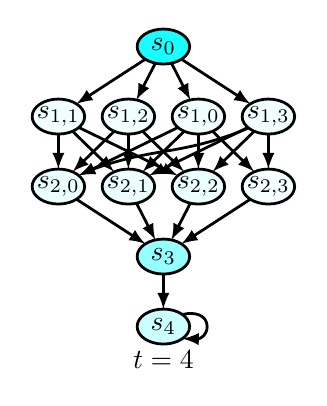
\begin{tikzpicture}[>=latex,line join=bevel,scale=0.35]
  \pgfsetlinewidth{1bp}
%%
\begin{scope}
  \definecolor{strokecol}{rgb}{0.0,0.0,0.0};
  \pgfsetstrokecolor{strokecol}
  \draw (135.0bp,16.0bp) node {$t=4$};
\end{scope}
  \pgfsetcolor{black}
  % Edge: s_{0} -> s_{1, 0}
  \draw [->] (143.35bp,320.76bp) .. controls (147.71bp,312.28bp) and (153.15bp,301.71bp)  .. (162.7bp,283.15bp);
  % Edge: s_{0} -> s_{1, 1}
  \draw [->] (116.19bp,324.81bp) .. controls (98.998bp,313.67bp) and (73.382bp,297.06bp)  .. (45.597bp,279.05bp);
  % Edge: s_{0} -> s_{1, 2}
  \draw [->] (126.65bp,320.76bp) .. controls (122.29bp,312.28bp) and (116.85bp,301.71bp)  .. (107.3bp,283.15bp);
  % Edge: s_{0} -> s_{1, 3}
  \draw [->] (153.81bp,324.81bp) .. controls (171.0bp,313.67bp) and (196.62bp,297.06bp)  .. (224.4bp,279.05bp);
  % Edge: s_{1, 0} -> s_{2, 0}
  \draw [->] (149.75bp,254.67bp) .. controls (125.4bp,242.83bp) and (85.281bp,223.33bp)  .. (48.335bp,205.37bp);
  % Edge: s_{1, 0} -> s_{2, 1}
  \draw [->] (156.43bp,250.83bp) .. controls (146.25bp,240.94bp) and (132.48bp,227.55bp)  .. (113.8bp,209.38bp);
  % Edge: s_{1, 0} -> s_{2, 2}
  \draw [->] (171.0bp,247.7bp) .. controls (171.0bp,239.98bp) and (171.0bp,230.71bp)  .. (171.0bp,212.1bp);
  % Edge: s_{1, 0} -> s_{2, 3}
  \draw [->] (185.57bp,250.83bp) .. controls (195.75bp,240.94bp) and (209.52bp,227.55bp)  .. (228.2bp,209.38bp);
  % Edge: s_{1, 1} -> s_{2, 0}
  \draw [->] (27.0bp,247.7bp) .. controls (27.0bp,239.98bp) and (27.0bp,230.71bp)  .. (27.0bp,212.1bp);
  % Edge: s_{1, 1} -> s_{2, 1}
  \draw [->] (41.57bp,250.83bp) .. controls (51.75bp,240.94bp) and (65.524bp,227.55bp)  .. (84.204bp,209.38bp);
  % Edge: s_{1, 1} -> s_{2, 2}
  \draw [->] (48.248bp,254.67bp) .. controls (72.602bp,242.83bp) and (112.72bp,223.33bp)  .. (149.67bp,205.37bp);
  % Edge: s_{1, 2} -> s_{2, 0}
  \draw [->] (84.43bp,250.83bp) .. controls (74.25bp,240.94bp) and (60.476bp,227.55bp)  .. (41.796bp,209.38bp);
  % Edge: s_{1, 2} -> s_{2, 1}
  \draw [->] (99.0bp,247.7bp) .. controls (99.0bp,239.98bp) and (99.0bp,230.71bp)  .. (99.0bp,212.1bp);
  % Edge: s_{1, 2} -> s_{2, 2}
  \draw [->] (113.57bp,250.83bp) .. controls (123.75bp,240.94bp) and (137.52bp,227.55bp)  .. (156.2bp,209.38bp);
  % Edge: s_{1, 3} -> s_{2, 0}
  \draw [->] (221.97bp,254.23bp) .. controls (217.13bp,251.98bp) and (211.95bp,249.77bp)  .. (207.0bp,248.0bp) .. controls (144.87bp,225.81bp) and (125.13bp,234.19bp)  .. (63.0bp,212.0bp) .. controls (61.145bp,211.34bp) and (59.257bp,210.61bp)  .. (48.028bp,205.77bp);
  % Edge: s_{1, 3} -> s_{2, 1}
  \draw [->] (221.75bp,254.67bp) .. controls (197.4bp,242.83bp) and (157.28bp,223.33bp)  .. (120.33bp,205.37bp);
  % Edge: s_{1, 3} -> s_{2, 2}
  \draw [->] (228.43bp,250.83bp) .. controls (218.25bp,240.94bp) and (204.48bp,227.55bp)  .. (185.8bp,209.38bp);
  % Edge: s_{1, 3} -> s_{2, 3}
  \draw [->] (243.0bp,247.7bp) .. controls (243.0bp,239.98bp) and (243.0bp,230.71bp)  .. (243.0bp,212.1bp);
  % Edge: s_{2, 0} -> s_{3}
  \draw [->] (45.812bp,180.81bp) .. controls (63.002bp,169.67bp) and (88.618bp,153.06bp)  .. (116.4bp,135.05bp);
  % Edge: s_{2, 1} -> s_{3}
  \draw [->] (107.35bp,176.76bp) .. controls (111.71bp,168.28bp) and (117.15bp,157.71bp)  .. (126.7bp,139.15bp);
  % Edge: s_{2, 2} -> s_{3}
  \draw [->] (162.65bp,176.76bp) .. controls (158.29bp,168.28bp) and (152.85bp,157.71bp)  .. (143.3bp,139.15bp);
  % Edge: s_{2, 3} -> s_{3}
  \draw [->] (224.19bp,180.81bp) .. controls (207.0bp,169.67bp) and (181.38bp,153.06bp)  .. (153.6bp,135.05bp);
  % Edge: s_{3} -> s_{4}
  \draw [->] (135.0bp,103.7bp) .. controls (135.0bp,95.983bp) and (135.0bp,86.712bp)  .. (135.0bp,68.104bp);
  % Edge: s_{4} -> s_{4}
  \draw [->] (154.9bp,62.432bp) .. controls (167.69bp,65.675bp) and (180.0bp,61.531bp)  .. (180.0bp,50.0bp) .. controls (180.0bp,41.622bp) and (173.5bp,37.143bp)  .. (154.9bp,37.568bp);
  % Node: s_{0}
\begin{scope}
  \definecolor{strokecol}{rgb}{0.0,0.0,0.0};
  \pgfsetstrokecolor{strokecol}
  \definecolor{fillcol}{rgb}{0.1,1.0,1.0};
  \pgfsetfillcolor{fillcol}
  \filldraw [opacity=1] (135.0bp,338.0bp) ellipse (27.0bp and 18.0bp);
  \draw (135.0bp,338.0bp) node {$s_{0}$};
\end{scope}
  % Node: s_{1, 0}
\begin{scope}
  \definecolor{strokecol}{rgb}{0.0,0.0,0.0};
  \pgfsetstrokecolor{strokecol}
  \definecolor{fillcol}{rgb}{0.95,1.0,1.0};
  \pgfsetfillcolor{fillcol}
  \filldraw [opacity=1] (171.0bp,266.0bp) ellipse (27.0bp and 18.0bp);
  \draw (171.0bp,266.0bp) node {$s_{1, 0}$};
\end{scope}
  % Node: s_{1, 1}
\begin{scope}
  \definecolor{strokecol}{rgb}{0.0,0.0,0.0};
  \pgfsetstrokecolor{strokecol}
  \definecolor{fillcol}{rgb}{0.95,1.0,1.0};
  \pgfsetfillcolor{fillcol}
  \filldraw [opacity=1] (27.0bp,266.0bp) ellipse (27.0bp and 18.0bp);
  \draw (27.0bp,266.0bp) node {$s_{1, 1}$};
\end{scope}
  % Node: s_{1, 2}
\begin{scope}
  \definecolor{strokecol}{rgb}{0.0,0.0,0.0};
  \pgfsetstrokecolor{strokecol}
  \definecolor{fillcol}{rgb}{0.95,1.0,1.0};
  \pgfsetfillcolor{fillcol}
  \filldraw [opacity=1] (99.0bp,266.0bp) ellipse (27.0bp and 18.0bp);
  \draw (99.0bp,266.0bp) node {$s_{1, 2}$};
\end{scope}
  % Node: s_{1, 3}
\begin{scope}
  \definecolor{strokecol}{rgb}{0.0,0.0,0.0};
  \pgfsetstrokecolor{strokecol}
  \definecolor{fillcol}{rgb}{0.95,1.0,1.0};
  \pgfsetfillcolor{fillcol}
  \filldraw [opacity=1] (243.0bp,266.0bp) ellipse (27.0bp and 18.0bp);
  \draw (243.0bp,266.0bp) node {$s_{1, 3}$};
\end{scope}
  % Node: s_{2, 0}
\begin{scope}
  \definecolor{strokecol}{rgb}{0.0,0.0,0.0};
  \pgfsetstrokecolor{strokecol}
  \definecolor{fillcol}{rgb}{0.92,1.0,1.0};
  \pgfsetfillcolor{fillcol}
  \filldraw [opacity=1] (27.0bp,194.0bp) ellipse (27.0bp and 18.0bp);
  \draw (27.0bp,194.0bp) node {$s_{2, 0}$};
\end{scope}
  % Node: s_{2, 1}
\begin{scope}
  \definecolor{strokecol}{rgb}{0.0,0.0,0.0};
  \pgfsetstrokecolor{strokecol}
  \definecolor{fillcol}{rgb}{0.92,1.0,1.0};
  \pgfsetfillcolor{fillcol}
  \filldraw [opacity=1] (99.0bp,194.0bp) ellipse (27.0bp and 18.0bp);
  \draw (99.0bp,194.0bp) node {$s_{2, 1}$};
\end{scope}
  % Node: s_{2, 2}
\begin{scope}
  \definecolor{strokecol}{rgb}{0.0,0.0,0.0};
  \pgfsetstrokecolor{strokecol}
  \definecolor{fillcol}{rgb}{0.92,1.0,1.0};
  \pgfsetfillcolor{fillcol}
  \filldraw [opacity=1] (171.0bp,194.0bp) ellipse (27.0bp and 18.0bp);
  \draw (171.0bp,194.0bp) node {$s_{2, 2}$};
\end{scope}
  % Node: s_{2, 3}
\begin{scope}
  \definecolor{strokecol}{rgb}{0.0,0.0,0.0};
  \pgfsetstrokecolor{strokecol}
  \definecolor{fillcol}{rgb}{0.96,1.0,1.0};
  \pgfsetfillcolor{fillcol}
  \filldraw [opacity=1] (243.0bp,194.0bp) ellipse (27.0bp and 18.0bp);
  \draw (243.0bp,194.0bp) node {$s_{2, 3}$};
\end{scope}
  % Node: s_{3}
\begin{scope}
  \definecolor{strokecol}{rgb}{0.0,0.0,0.0};
  \pgfsetstrokecolor{strokecol}
  \definecolor{fillcol}{rgb}{0.59,1.0,1.0};
  \pgfsetfillcolor{fillcol}
  \filldraw [opacity=1] (135.0bp,122.0bp) ellipse (27.0bp and 18.0bp);
  \draw (135.0bp,122.0bp) node {$s_{3}$};
\end{scope}
  % Node: s_{4}
\begin{scope}
  \definecolor{strokecol}{rgb}{0.0,0.0,0.0};
  \pgfsetstrokecolor{strokecol}
  \definecolor{fillcol}{rgb}{0.8,1.0,1.0};
  \pgfsetfillcolor{fillcol}
  \filldraw [opacity=1] (135.0bp,50.0bp) ellipse (27.0bp and 18.0bp);
  \draw (135.0bp,50.0bp) node {$s_{4}$};
\end{scope}
%
\end{tikzpicture}
    
        \end{minipage}
        \begin{minipage}{.24\textwidth}
        
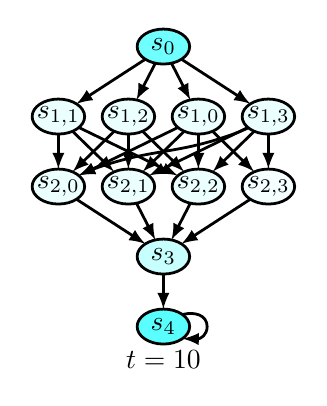
\begin{tikzpicture}[>=latex,line join=bevel,scale=0.35]
  \pgfsetlinewidth{1bp}
%%
\begin{scope}
  \definecolor{strokecol}{rgb}{0.0,0.0,0.0};
  \pgfsetstrokecolor{strokecol}
  \draw (135.0bp,16.0bp) node {$t=10$};
\end{scope}
  \pgfsetcolor{black}
  % Edge: s_{0} -> s_{1, 0}
  \draw [->] (143.35bp,320.76bp) .. controls (147.71bp,312.28bp) and (153.15bp,301.71bp)  .. (162.7bp,283.15bp);
  % Edge: s_{0} -> s_{1, 1}
  \draw [->] (116.19bp,324.81bp) .. controls (98.998bp,313.67bp) and (73.382bp,297.06bp)  .. (45.597bp,279.05bp);
  % Edge: s_{0} -> s_{1, 2}
  \draw [->] (126.65bp,320.76bp) .. controls (122.29bp,312.28bp) and (116.85bp,301.71bp)  .. (107.3bp,283.15bp);
  % Edge: s_{0} -> s_{1, 3}
  \draw [->] (153.81bp,324.81bp) .. controls (171.0bp,313.67bp) and (196.62bp,297.06bp)  .. (224.4bp,279.05bp);
  % Edge: s_{1, 0} -> s_{2, 0}
  \draw [->] (149.75bp,254.67bp) .. controls (125.4bp,242.83bp) and (85.281bp,223.33bp)  .. (48.335bp,205.37bp);
  % Edge: s_{1, 0} -> s_{2, 1}
  \draw [->] (156.43bp,250.83bp) .. controls (146.25bp,240.94bp) and (132.48bp,227.55bp)  .. (113.8bp,209.38bp);
  % Edge: s_{1, 0} -> s_{2, 2}
  \draw [->] (171.0bp,247.7bp) .. controls (171.0bp,239.98bp) and (171.0bp,230.71bp)  .. (171.0bp,212.1bp);
  % Edge: s_{1, 0} -> s_{2, 3}
  \draw [->] (185.57bp,250.83bp) .. controls (195.75bp,240.94bp) and (209.52bp,227.55bp)  .. (228.2bp,209.38bp);
  % Edge: s_{1, 1} -> s_{2, 0}
  \draw [->] (27.0bp,247.7bp) .. controls (27.0bp,239.98bp) and (27.0bp,230.71bp)  .. (27.0bp,212.1bp);
  % Edge: s_{1, 1} -> s_{2, 1}
  \draw [->] (41.57bp,250.83bp) .. controls (51.75bp,240.94bp) and (65.524bp,227.55bp)  .. (84.204bp,209.38bp);
  % Edge: s_{1, 1} -> s_{2, 2}
  \draw [->] (48.248bp,254.67bp) .. controls (72.602bp,242.83bp) and (112.72bp,223.33bp)  .. (149.67bp,205.37bp);
  % Edge: s_{1, 2} -> s_{2, 0}
  \draw [->] (84.43bp,250.83bp) .. controls (74.25bp,240.94bp) and (60.476bp,227.55bp)  .. (41.796bp,209.38bp);
  % Edge: s_{1, 2} -> s_{2, 1}
  \draw [->] (99.0bp,247.7bp) .. controls (99.0bp,239.98bp) and (99.0bp,230.71bp)  .. (99.0bp,212.1bp);
  % Edge: s_{1, 2} -> s_{2, 2}
  \draw [->] (113.57bp,250.83bp) .. controls (123.75bp,240.94bp) and (137.52bp,227.55bp)  .. (156.2bp,209.38bp);
  % Edge: s_{1, 3} -> s_{2, 0}
  \draw [->] (221.97bp,254.23bp) .. controls (217.13bp,251.98bp) and (211.95bp,249.77bp)  .. (207.0bp,248.0bp) .. controls (144.87bp,225.81bp) and (125.13bp,234.19bp)  .. (63.0bp,212.0bp) .. controls (61.145bp,211.34bp) and (59.257bp,210.61bp)  .. (48.028bp,205.77bp);
  % Edge: s_{1, 3} -> s_{2, 1}
  \draw [->] (221.75bp,254.67bp) .. controls (197.4bp,242.83bp) and (157.28bp,223.33bp)  .. (120.33bp,205.37bp);
  % Edge: s_{1, 3} -> s_{2, 2}
  \draw [->] (228.43bp,250.83bp) .. controls (218.25bp,240.94bp) and (204.48bp,227.55bp)  .. (185.8bp,209.38bp);
  % Edge: s_{1, 3} -> s_{2, 3}
  \draw [->] (243.0bp,247.7bp) .. controls (243.0bp,239.98bp) and (243.0bp,230.71bp)  .. (243.0bp,212.1bp);
  % Edge: s_{2, 0} -> s_{3}
  \draw [->] (45.812bp,180.81bp) .. controls (63.002bp,169.67bp) and (88.618bp,153.06bp)  .. (116.4bp,135.05bp);
  % Edge: s_{2, 1} -> s_{3}
  \draw [->] (107.35bp,176.76bp) .. controls (111.71bp,168.28bp) and (117.15bp,157.71bp)  .. (126.7bp,139.15bp);
  % Edge: s_{2, 2} -> s_{3}
  \draw [->] (162.65bp,176.76bp) .. controls (158.29bp,168.28bp) and (152.85bp,157.71bp)  .. (143.3bp,139.15bp);
  % Edge: s_{2, 3} -> s_{3}
  \draw [->] (224.19bp,180.81bp) .. controls (207.0bp,169.67bp) and (181.38bp,153.06bp)  .. (153.6bp,135.05bp);
  % Edge: s_{3} -> s_{4}
  \draw [->] (135.0bp,103.7bp) .. controls (135.0bp,95.983bp) and (135.0bp,86.712bp)  .. (135.0bp,68.104bp);
  % Edge: s_{4} -> s_{4}
  \draw [->] (154.9bp,62.432bp) .. controls (167.69bp,65.675bp) and (180.0bp,61.531bp)  .. (180.0bp,50.0bp) .. controls (180.0bp,41.622bp) and (173.5bp,37.143bp)  .. (154.9bp,37.568bp);
  % Node: s_{0}
\begin{scope}
  \definecolor{strokecol}{rgb}{0.0,0.0,0.0};
  \pgfsetstrokecolor{strokecol}
  \definecolor{fillcol}{rgb}{0.44,1.0,1.0};
  \pgfsetfillcolor{fillcol}
  \filldraw [opacity=1] (135.0bp,338.0bp) ellipse (27.0bp and 18.0bp);
  \draw (135.0bp,338.0bp) node {$s_{0}$};
\end{scope}
  % Node: s_{1, 0}
\begin{scope}
  \definecolor{strokecol}{rgb}{0.0,0.0,0.0};
  \pgfsetstrokecolor{strokecol}
  \definecolor{fillcol}{rgb}{0.92,1.0,1.0};
  \pgfsetfillcolor{fillcol}
  \filldraw [opacity=1] (171.0bp,266.0bp) ellipse (27.0bp and 18.0bp);
  \draw (171.0bp,266.0bp) node {$s_{1, 0}$};
\end{scope}
  % Node: s_{1, 1}
\begin{scope}
  \definecolor{strokecol}{rgb}{0.0,0.0,0.0};
  \pgfsetstrokecolor{strokecol}
  \definecolor{fillcol}{rgb}{0.92,1.0,1.0};
  \pgfsetfillcolor{fillcol}
  \filldraw [opacity=1] (27.0bp,266.0bp) ellipse (27.0bp and 18.0bp);
  \draw (27.0bp,266.0bp) node {$s_{1, 1}$};
\end{scope}
  % Node: s_{1, 2}
\begin{scope}
  \definecolor{strokecol}{rgb}{0.0,0.0,0.0};
  \pgfsetstrokecolor{strokecol}
  \definecolor{fillcol}{rgb}{0.92,1.0,1.0};
  \pgfsetfillcolor{fillcol}
  \filldraw [opacity=1] (99.0bp,266.0bp) ellipse (27.0bp and 18.0bp);
  \draw (99.0bp,266.0bp) node {$s_{1, 2}$};
\end{scope}
  % Node: s_{1, 3}
\begin{scope}
  \definecolor{strokecol}{rgb}{0.0,0.0,0.0};
  \pgfsetstrokecolor{strokecol}
  \definecolor{fillcol}{rgb}{0.92,1.0,1.0};
  \pgfsetfillcolor{fillcol}
  \filldraw [opacity=1] (243.0bp,266.0bp) ellipse (27.0bp and 18.0bp);
  \draw (243.0bp,266.0bp) node {$s_{1, 3}$};
\end{scope}
  % Node: s_{2, 0}
\begin{scope}
  \definecolor{strokecol}{rgb}{0.0,0.0,0.0};
  \pgfsetstrokecolor{strokecol}
  \definecolor{fillcol}{rgb}{0.92,1.0,1.0};
  \pgfsetfillcolor{fillcol}
  \filldraw [opacity=1] (27.0bp,194.0bp) ellipse (27.0bp and 18.0bp);
  \draw (27.0bp,194.0bp) node {$s_{2, 0}$};
\end{scope}
  % Node: s_{2, 1}
\begin{scope}
  \definecolor{strokecol}{rgb}{0.0,0.0,0.0};
  \pgfsetstrokecolor{strokecol}
  \definecolor{fillcol}{rgb}{0.92,1.0,1.0};
  \pgfsetfillcolor{fillcol}
  \filldraw [opacity=1] (99.0bp,194.0bp) ellipse (27.0bp and 18.0bp);
  \draw (99.0bp,194.0bp) node {$s_{2, 1}$};
\end{scope}
  % Node: s_{2, 2}
\begin{scope}
  \definecolor{strokecol}{rgb}{0.0,0.0,0.0};
  \pgfsetstrokecolor{strokecol}
  \definecolor{fillcol}{rgb}{0.92,1.0,1.0};
  \pgfsetfillcolor{fillcol}
  \filldraw [opacity=1] (171.0bp,194.0bp) ellipse (27.0bp and 18.0bp);
  \draw (171.0bp,194.0bp) node {$s_{2, 2}$};
\end{scope}
  % Node: s_{2, 3}
\begin{scope}
  \definecolor{strokecol}{rgb}{0.0,0.0,0.0};
  \pgfsetstrokecolor{strokecol}
  \definecolor{fillcol}{rgb}{0.96,1.0,1.0};
  \pgfsetfillcolor{fillcol}
  \filldraw [opacity=1] (243.0bp,194.0bp) ellipse (27.0bp and 18.0bp);
  \draw (243.0bp,194.0bp) node {$s_{2, 3}$};
\end{scope}
  % Node: s_{3}
\begin{scope}
  \definecolor{strokecol}{rgb}{0.0,0.0,0.0};
  \pgfsetstrokecolor{strokecol}
  \definecolor{fillcol}{rgb}{0.78,1.0,1.0};
  \pgfsetfillcolor{fillcol}
  \filldraw [opacity=1] (135.0bp,122.0bp) ellipse (27.0bp and 18.0bp);
  \draw (135.0bp,122.0bp) node {$s_{3}$};
\end{scope}
  % Node: s_{4}
\begin{scope}
  \definecolor{strokecol}{rgb}{0.0,0.0,0.0};
  \pgfsetstrokecolor{strokecol}
  \definecolor{fillcol}{rgb}{0.35,1.0,1.0};
  \pgfsetfillcolor{fillcol}
  \filldraw [opacity=1] (135.0bp,50.0bp) ellipse (27.0bp and 18.0bp);
  \draw (135.0bp,50.0bp) node {$s_{4}$};
\end{scope}
%
\end{tikzpicture}
    
        \end{minipage}
        \begin{minipage}{.24\textwidth}
        
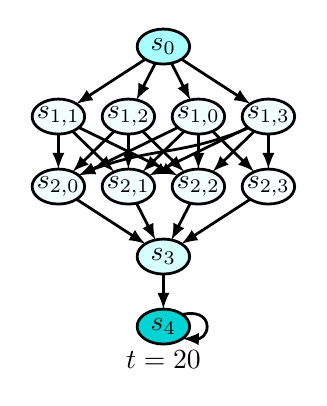
\begin{tikzpicture}[>=latex,line join=bevel,scale=0.35]
  \pgfsetlinewidth{1bp}
%%
\begin{scope}
  \definecolor{strokecol}{rgb}{0.0,0.0,0.0};
  \pgfsetstrokecolor{strokecol}
  \draw (135.0bp,16.0bp) node {$t=20$};
\end{scope}
  \pgfsetcolor{black}
  % Edge: s_{0} -> s_{1, 0}
  \draw [->] (143.35bp,320.76bp) .. controls (147.71bp,312.28bp) and (153.15bp,301.71bp)  .. (162.7bp,283.15bp);
  % Edge: s_{0} -> s_{1, 1}
  \draw [->] (116.19bp,324.81bp) .. controls (98.998bp,313.67bp) and (73.382bp,297.06bp)  .. (45.597bp,279.05bp);
  % Edge: s_{0} -> s_{1, 2}
  \draw [->] (126.65bp,320.76bp) .. controls (122.29bp,312.28bp) and (116.85bp,301.71bp)  .. (107.3bp,283.15bp);
  % Edge: s_{0} -> s_{1, 3}
  \draw [->] (153.81bp,324.81bp) .. controls (171.0bp,313.67bp) and (196.62bp,297.06bp)  .. (224.4bp,279.05bp);
  % Edge: s_{1, 0} -> s_{2, 0}
  \draw [->] (149.75bp,254.67bp) .. controls (125.4bp,242.83bp) and (85.281bp,223.33bp)  .. (48.335bp,205.37bp);
  % Edge: s_{1, 0} -> s_{2, 1}
  \draw [->] (156.43bp,250.83bp) .. controls (146.25bp,240.94bp) and (132.48bp,227.55bp)  .. (113.8bp,209.38bp);
  % Edge: s_{1, 0} -> s_{2, 2}
  \draw [->] (171.0bp,247.7bp) .. controls (171.0bp,239.98bp) and (171.0bp,230.71bp)  .. (171.0bp,212.1bp);
  % Edge: s_{1, 0} -> s_{2, 3}
  \draw [->] (185.57bp,250.83bp) .. controls (195.75bp,240.94bp) and (209.52bp,227.55bp)  .. (228.2bp,209.38bp);
  % Edge: s_{1, 1} -> s_{2, 0}
  \draw [->] (27.0bp,247.7bp) .. controls (27.0bp,239.98bp) and (27.0bp,230.71bp)  .. (27.0bp,212.1bp);
  % Edge: s_{1, 1} -> s_{2, 1}
  \draw [->] (41.57bp,250.83bp) .. controls (51.75bp,240.94bp) and (65.524bp,227.55bp)  .. (84.204bp,209.38bp);
  % Edge: s_{1, 1} -> s_{2, 2}
  \draw [->] (48.248bp,254.67bp) .. controls (72.602bp,242.83bp) and (112.72bp,223.33bp)  .. (149.67bp,205.37bp);
  % Edge: s_{1, 2} -> s_{2, 0}
  \draw [->] (84.43bp,250.83bp) .. controls (74.25bp,240.94bp) and (60.476bp,227.55bp)  .. (41.796bp,209.38bp);
  % Edge: s_{1, 2} -> s_{2, 1}
  \draw [->] (99.0bp,247.7bp) .. controls (99.0bp,239.98bp) and (99.0bp,230.71bp)  .. (99.0bp,212.1bp);
  % Edge: s_{1, 2} -> s_{2, 2}
  \draw [->] (113.57bp,250.83bp) .. controls (123.75bp,240.94bp) and (137.52bp,227.55bp)  .. (156.2bp,209.38bp);
  % Edge: s_{1, 3} -> s_{2, 0}
  \draw [->] (221.97bp,254.23bp) .. controls (217.13bp,251.98bp) and (211.95bp,249.77bp)  .. (207.0bp,248.0bp) .. controls (144.87bp,225.81bp) and (125.13bp,234.19bp)  .. (63.0bp,212.0bp) .. controls (61.145bp,211.34bp) and (59.257bp,210.61bp)  .. (48.028bp,205.77bp);
  % Edge: s_{1, 3} -> s_{2, 1}
  \draw [->] (221.75bp,254.67bp) .. controls (197.4bp,242.83bp) and (157.28bp,223.33bp)  .. (120.33bp,205.37bp);
  % Edge: s_{1, 3} -> s_{2, 2}
  \draw [->] (228.43bp,250.83bp) .. controls (218.25bp,240.94bp) and (204.48bp,227.55bp)  .. (185.8bp,209.38bp);
  % Edge: s_{1, 3} -> s_{2, 3}
  \draw [->] (243.0bp,247.7bp) .. controls (243.0bp,239.98bp) and (243.0bp,230.71bp)  .. (243.0bp,212.1bp);
  % Edge: s_{2, 0} -> s_{3}
  \draw [->] (45.812bp,180.81bp) .. controls (63.002bp,169.67bp) and (88.618bp,153.06bp)  .. (116.4bp,135.05bp);
  % Edge: s_{2, 1} -> s_{3}
  \draw [->] (107.35bp,176.76bp) .. controls (111.71bp,168.28bp) and (117.15bp,157.71bp)  .. (126.7bp,139.15bp);
  % Edge: s_{2, 2} -> s_{3}
  \draw [->] (162.65bp,176.76bp) .. controls (158.29bp,168.28bp) and (152.85bp,157.71bp)  .. (143.3bp,139.15bp);
  % Edge: s_{2, 3} -> s_{3}
  \draw [->] (224.19bp,180.81bp) .. controls (207.0bp,169.67bp) and (181.38bp,153.06bp)  .. (153.6bp,135.05bp);
  % Edge: s_{3} -> s_{4}
  \draw [->] (135.0bp,103.7bp) .. controls (135.0bp,95.983bp) and (135.0bp,86.712bp)  .. (135.0bp,68.104bp);
  % Edge: s_{4} -> s_{4}
  \draw [->] (154.9bp,62.432bp) .. controls (167.69bp,65.675bp) and (180.0bp,61.531bp)  .. (180.0bp,50.0bp) .. controls (180.0bp,41.622bp) and (173.5bp,37.143bp)  .. (154.9bp,37.568bp);
  % Node: s_{0}
\begin{scope}
  \definecolor{strokecol}{rgb}{0.0,0.0,0.0};
  \pgfsetstrokecolor{strokecol}
  \definecolor{fillcol}{rgb}{0.66,1.0,1.0};
  \pgfsetfillcolor{fillcol}
  \filldraw [opacity=1] (135.0bp,338.0bp) ellipse (27.0bp and 18.0bp);
  \draw (135.0bp,338.0bp) node {$s_{0}$};
\end{scope}
  % Node: s_{1, 0}
\begin{scope}
  \definecolor{strokecol}{rgb}{0.0,0.0,0.0};
  \pgfsetstrokecolor{strokecol}
  \definecolor{fillcol}{rgb}{0.95,1.0,1.0};
  \pgfsetfillcolor{fillcol}
  \filldraw [opacity=1] (171.0bp,266.0bp) ellipse (27.0bp and 18.0bp);
  \draw (171.0bp,266.0bp) node {$s_{1, 0}$};
\end{scope}
  % Node: s_{1, 1}
\begin{scope}
  \definecolor{strokecol}{rgb}{0.0,0.0,0.0};
  \pgfsetstrokecolor{strokecol}
  \definecolor{fillcol}{rgb}{0.95,1.0,1.0};
  \pgfsetfillcolor{fillcol}
  \filldraw [opacity=1] (27.0bp,266.0bp) ellipse (27.0bp and 18.0bp);
  \draw (27.0bp,266.0bp) node {$s_{1, 1}$};
\end{scope}
  % Node: s_{1, 2}
\begin{scope}
  \definecolor{strokecol}{rgb}{0.0,0.0,0.0};
  \pgfsetstrokecolor{strokecol}
  \definecolor{fillcol}{rgb}{0.95,1.0,1.0};
  \pgfsetfillcolor{fillcol}
  \filldraw [opacity=1] (99.0bp,266.0bp) ellipse (27.0bp and 18.0bp);
  \draw (99.0bp,266.0bp) node {$s_{1, 2}$};
\end{scope}
  % Node: s_{1, 3}
\begin{scope}
  \definecolor{strokecol}{rgb}{0.0,0.0,0.0};
  \pgfsetstrokecolor{strokecol}
  \definecolor{fillcol}{rgb}{0.95,1.0,1.0};
  \pgfsetfillcolor{fillcol}
  \filldraw [opacity=1] (243.0bp,266.0bp) ellipse (27.0bp and 18.0bp);
  \draw (243.0bp,266.0bp) node {$s_{1, 3}$};
\end{scope}
  % Node: s_{2, 0}
\begin{scope}
  \definecolor{strokecol}{rgb}{0.0,0.0,0.0};
  \pgfsetstrokecolor{strokecol}
  \definecolor{fillcol}{rgb}{0.95,1.0,1.0};
  \pgfsetfillcolor{fillcol}
  \filldraw [opacity=1] (27.0bp,194.0bp) ellipse (27.0bp and 18.0bp);
  \draw (27.0bp,194.0bp) node {$s_{2, 0}$};
\end{scope}
  % Node: s_{2, 1}
\begin{scope}
  \definecolor{strokecol}{rgb}{0.0,0.0,0.0};
  \pgfsetstrokecolor{strokecol}
  \definecolor{fillcol}{rgb}{0.95,1.0,1.0};
  \pgfsetfillcolor{fillcol}
  \filldraw [opacity=1] (99.0bp,194.0bp) ellipse (27.0bp and 18.0bp);
  \draw (99.0bp,194.0bp) node {$s_{2, 1}$};
\end{scope}
  % Node: s_{2, 2}
\begin{scope}
  \definecolor{strokecol}{rgb}{0.0,0.0,0.0};
  \pgfsetstrokecolor{strokecol}
  \definecolor{fillcol}{rgb}{0.95,1.0,1.0};
  \pgfsetfillcolor{fillcol}
  \filldraw [opacity=1] (171.0bp,194.0bp) ellipse (27.0bp and 18.0bp);
  \draw (171.0bp,194.0bp) node {$s_{2, 2}$};
\end{scope}
  % Node: s_{2, 3}
\begin{scope}
  \definecolor{strokecol}{rgb}{0.0,0.0,0.0};
  \pgfsetstrokecolor{strokecol}
  \definecolor{fillcol}{rgb}{0.98,1.0,1.0};
  \pgfsetfillcolor{fillcol}
  \filldraw [opacity=1] (243.0bp,194.0bp) ellipse (27.0bp and 18.0bp);
  \draw (243.0bp,194.0bp) node {$s_{2, 3}$};
\end{scope}
  % Node: s_{3}
\begin{scope}
  \definecolor{strokecol}{rgb}{0.0,0.0,0.0};
  \pgfsetstrokecolor{strokecol}
  \definecolor{fillcol}{rgb}{0.84,1.0,1.0};
  \pgfsetfillcolor{fillcol}
  \filldraw [opacity=1] (135.0bp,122.0bp) ellipse (27.0bp and 18.0bp);
  \draw (135.0bp,122.0bp) node {$s_{3}$};
\end{scope}
  % Node: s_{4}
\begin{scope}
  \definecolor{strokecol}{rgb}{0.0,0.0,0.0};
  \pgfsetstrokecolor{strokecol}
  \definecolor{fillcol}{rgb}{0.0,0.83,0.83};
  \pgfsetfillcolor{fillcol}
  \filldraw [opacity=1] (135.0bp,50.0bp) ellipse (27.0bp and 18.0bp);
  \draw (135.0bp,50.0bp) node {$s_{4}$};
\end{scope}
%
\end{tikzpicture}
    
        \end{minipage}
        \begin{minipage}{.24\textwidth}
        
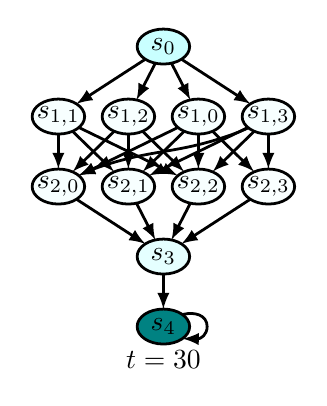
\begin{tikzpicture}[>=latex,line join=bevel,scale=0.35]
  \pgfsetlinewidth{1bp}
%%
\begin{scope}
  \definecolor{strokecol}{rgb}{0.0,0.0,0.0};
  \pgfsetstrokecolor{strokecol}
  \draw (135.0bp,16.0bp) node {$t=30$};
\end{scope}
  \pgfsetcolor{black}
  % Edge: s_{0} -> s_{1, 0}
  \draw [->] (143.35bp,320.76bp) .. controls (147.71bp,312.28bp) and (153.15bp,301.71bp)  .. (162.7bp,283.15bp);
  % Edge: s_{0} -> s_{1, 1}
  \draw [->] (116.19bp,324.81bp) .. controls (98.998bp,313.67bp) and (73.382bp,297.06bp)  .. (45.597bp,279.05bp);
  % Edge: s_{0} -> s_{1, 2}
  \draw [->] (126.65bp,320.76bp) .. controls (122.29bp,312.28bp) and (116.85bp,301.71bp)  .. (107.3bp,283.15bp);
  % Edge: s_{0} -> s_{1, 3}
  \draw [->] (153.81bp,324.81bp) .. controls (171.0bp,313.67bp) and (196.62bp,297.06bp)  .. (224.4bp,279.05bp);
  % Edge: s_{1, 0} -> s_{2, 0}
  \draw [->] (149.75bp,254.67bp) .. controls (125.4bp,242.83bp) and (85.281bp,223.33bp)  .. (48.335bp,205.37bp);
  % Edge: s_{1, 0} -> s_{2, 1}
  \draw [->] (156.43bp,250.83bp) .. controls (146.25bp,240.94bp) and (132.48bp,227.55bp)  .. (113.8bp,209.38bp);
  % Edge: s_{1, 0} -> s_{2, 2}
  \draw [->] (171.0bp,247.7bp) .. controls (171.0bp,239.98bp) and (171.0bp,230.71bp)  .. (171.0bp,212.1bp);
  % Edge: s_{1, 0} -> s_{2, 3}
  \draw [->] (185.57bp,250.83bp) .. controls (195.75bp,240.94bp) and (209.52bp,227.55bp)  .. (228.2bp,209.38bp);
  % Edge: s_{1, 1} -> s_{2, 0}
  \draw [->] (27.0bp,247.7bp) .. controls (27.0bp,239.98bp) and (27.0bp,230.71bp)  .. (27.0bp,212.1bp);
  % Edge: s_{1, 1} -> s_{2, 1}
  \draw [->] (41.57bp,250.83bp) .. controls (51.75bp,240.94bp) and (65.524bp,227.55bp)  .. (84.204bp,209.38bp);
  % Edge: s_{1, 1} -> s_{2, 2}
  \draw [->] (48.248bp,254.67bp) .. controls (72.602bp,242.83bp) and (112.72bp,223.33bp)  .. (149.67bp,205.37bp);
  % Edge: s_{1, 2} -> s_{2, 0}
  \draw [->] (84.43bp,250.83bp) .. controls (74.25bp,240.94bp) and (60.476bp,227.55bp)  .. (41.796bp,209.38bp);
  % Edge: s_{1, 2} -> s_{2, 1}
  \draw [->] (99.0bp,247.7bp) .. controls (99.0bp,239.98bp) and (99.0bp,230.71bp)  .. (99.0bp,212.1bp);
  % Edge: s_{1, 2} -> s_{2, 2}
  \draw [->] (113.57bp,250.83bp) .. controls (123.75bp,240.94bp) and (137.52bp,227.55bp)  .. (156.2bp,209.38bp);
  % Edge: s_{1, 3} -> s_{2, 0}
  \draw [->] (221.97bp,254.23bp) .. controls (217.13bp,251.98bp) and (211.95bp,249.77bp)  .. (207.0bp,248.0bp) .. controls (144.87bp,225.81bp) and (125.13bp,234.19bp)  .. (63.0bp,212.0bp) .. controls (61.145bp,211.34bp) and (59.257bp,210.61bp)  .. (48.028bp,205.77bp);
  % Edge: s_{1, 3} -> s_{2, 1}
  \draw [->] (221.75bp,254.67bp) .. controls (197.4bp,242.83bp) and (157.28bp,223.33bp)  .. (120.33bp,205.37bp);
  % Edge: s_{1, 3} -> s_{2, 2}
  \draw [->] (228.43bp,250.83bp) .. controls (218.25bp,240.94bp) and (204.48bp,227.55bp)  .. (185.8bp,209.38bp);
  % Edge: s_{1, 3} -> s_{2, 3}
  \draw [->] (243.0bp,247.7bp) .. controls (243.0bp,239.98bp) and (243.0bp,230.71bp)  .. (243.0bp,212.1bp);
  % Edge: s_{2, 0} -> s_{3}
  \draw [->] (45.812bp,180.81bp) .. controls (63.002bp,169.67bp) and (88.618bp,153.06bp)  .. (116.4bp,135.05bp);
  % Edge: s_{2, 1} -> s_{3}
  \draw [->] (107.35bp,176.76bp) .. controls (111.71bp,168.28bp) and (117.15bp,157.71bp)  .. (126.7bp,139.15bp);
  % Edge: s_{2, 2} -> s_{3}
  \draw [->] (162.65bp,176.76bp) .. controls (158.29bp,168.28bp) and (152.85bp,157.71bp)  .. (143.3bp,139.15bp);
  % Edge: s_{2, 3} -> s_{3}
  \draw [->] (224.19bp,180.81bp) .. controls (207.0bp,169.67bp) and (181.38bp,153.06bp)  .. (153.6bp,135.05bp);
  % Edge: s_{3} -> s_{4}
  \draw [->] (135.0bp,103.7bp) .. controls (135.0bp,95.983bp) and (135.0bp,86.712bp)  .. (135.0bp,68.104bp);
  % Edge: s_{4} -> s_{4}
  \draw [->] (154.9bp,62.432bp) .. controls (167.69bp,65.675bp) and (180.0bp,61.531bp)  .. (180.0bp,50.0bp) .. controls (180.0bp,41.622bp) and (173.5bp,37.143bp)  .. (154.9bp,37.568bp);
  % Node: s_{0}
\begin{scope}
  \definecolor{strokecol}{rgb}{0.0,0.0,0.0};
  \pgfsetstrokecolor{strokecol}
  \definecolor{fillcol}{rgb}{0.79,1.0,1.0};
  \pgfsetfillcolor{fillcol}
  \filldraw [opacity=1] (135.0bp,338.0bp) ellipse (27.0bp and 18.0bp);
  \draw (135.0bp,338.0bp) node {$s_{0}$};
\end{scope}
  % Node: s_{1, 0}
\begin{scope}
  \definecolor{strokecol}{rgb}{0.0,0.0,0.0};
  \pgfsetstrokecolor{strokecol}
  \definecolor{fillcol}{rgb}{0.97,1.0,1.0};
  \pgfsetfillcolor{fillcol}
  \filldraw [opacity=1] (171.0bp,266.0bp) ellipse (27.0bp and 18.0bp);
  \draw (171.0bp,266.0bp) node {$s_{1, 0}$};
\end{scope}
  % Node: s_{1, 1}
\begin{scope}
  \definecolor{strokecol}{rgb}{0.0,0.0,0.0};
  \pgfsetstrokecolor{strokecol}
  \definecolor{fillcol}{rgb}{0.97,1.0,1.0};
  \pgfsetfillcolor{fillcol}
  \filldraw [opacity=1] (27.0bp,266.0bp) ellipse (27.0bp and 18.0bp);
  \draw (27.0bp,266.0bp) node {$s_{1, 1}$};
\end{scope}
  % Node: s_{1, 2}
\begin{scope}
  \definecolor{strokecol}{rgb}{0.0,0.0,0.0};
  \pgfsetstrokecolor{strokecol}
  \definecolor{fillcol}{rgb}{0.97,1.0,1.0};
  \pgfsetfillcolor{fillcol}
  \filldraw [opacity=1] (99.0bp,266.0bp) ellipse (27.0bp and 18.0bp);
  \draw (99.0bp,266.0bp) node {$s_{1, 2}$};
\end{scope}
  % Node: s_{1, 3}
\begin{scope}
  \definecolor{strokecol}{rgb}{0.0,0.0,0.0};
  \pgfsetstrokecolor{strokecol}
  \definecolor{fillcol}{rgb}{0.97,1.0,1.0};
  \pgfsetfillcolor{fillcol}
  \filldraw [opacity=1] (243.0bp,266.0bp) ellipse (27.0bp and 18.0bp);
  \draw (243.0bp,266.0bp) node {$s_{1, 3}$};
\end{scope}
  % Node: s_{2, 0}
\begin{scope}
  \definecolor{strokecol}{rgb}{0.0,0.0,0.0};
  \pgfsetstrokecolor{strokecol}
  \definecolor{fillcol}{rgb}{0.97,1.0,1.0};
  \pgfsetfillcolor{fillcol}
  \filldraw [opacity=1] (27.0bp,194.0bp) ellipse (27.0bp and 18.0bp);
  \draw (27.0bp,194.0bp) node {$s_{2, 0}$};
\end{scope}
  % Node: s_{2, 1}
\begin{scope}
  \definecolor{strokecol}{rgb}{0.0,0.0,0.0};
  \pgfsetstrokecolor{strokecol}
  \definecolor{fillcol}{rgb}{0.97,1.0,1.0};
  \pgfsetfillcolor{fillcol}
  \filldraw [opacity=1] (99.0bp,194.0bp) ellipse (27.0bp and 18.0bp);
  \draw (99.0bp,194.0bp) node {$s_{2, 1}$};
\end{scope}
  % Node: s_{2, 2}
\begin{scope}
  \definecolor{strokecol}{rgb}{0.0,0.0,0.0};
  \pgfsetstrokecolor{strokecol}
  \definecolor{fillcol}{rgb}{0.97,1.0,1.0};
  \pgfsetfillcolor{fillcol}
  \filldraw [opacity=1] (171.0bp,194.0bp) ellipse (27.0bp and 18.0bp);
  \draw (171.0bp,194.0bp) node {$s_{2, 2}$};
\end{scope}
  % Node: s_{2, 3}
\begin{scope}
  \definecolor{strokecol}{rgb}{0.0,0.0,0.0};
  \pgfsetstrokecolor{strokecol}
  \definecolor{fillcol}{rgb}{0.98,1.0,1.0};
  \pgfsetfillcolor{fillcol}
  \filldraw [opacity=1] (243.0bp,194.0bp) ellipse (27.0bp and 18.0bp);
  \draw (243.0bp,194.0bp) node {$s_{2, 3}$};
\end{scope}
  % Node: s_{3}
\begin{scope}
  \definecolor{strokecol}{rgb}{0.0,0.0,0.0};
  \pgfsetstrokecolor{strokecol}
  \definecolor{fillcol}{rgb}{0.9,1.0,1.0};
  \pgfsetfillcolor{fillcol}
  \filldraw [opacity=1] (135.0bp,122.0bp) ellipse (27.0bp and 18.0bp);
  \draw (135.0bp,122.0bp) node {$s_{3}$};
\end{scope}
  % Node: s_{4}
\begin{scope}
  \definecolor{strokecol}{rgb}{0.0,0.0,0.0};
  \pgfsetstrokecolor{strokecol}
  \definecolor{fillcol}{rgb}{0.0,0.51,0.51};
  \pgfsetfillcolor{fillcol}
  \filldraw [opacity=1] (135.0bp,50.0bp) ellipse (27.0bp and 18.0bp);
  \draw (135.0bp,50.0bp) node {$s_{4}$};
\end{scope}
%
\end{tikzpicture}
    
        \end{minipage}
        \caption{Distribution of states at time step $t$ for $n=4$, $m=4$. Darker means higher probability}
        \label{fig:distmc}
    \end{center}
\end{figure}

\begin{figure}
    \begin{center}
        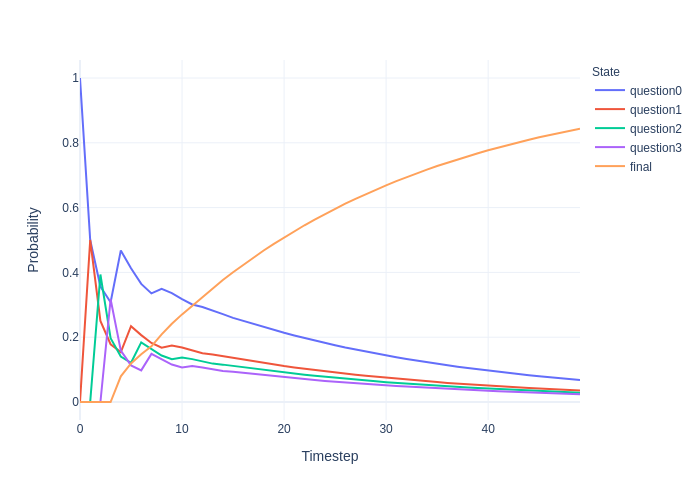
\includegraphics[scale=0.5]{imgs/dist_questions.png}
        \caption{Probability of being at each question over time}
        \label{fig:dist_questions}
    \end{center}
\end{figure}


\subsection{Optimality of the greedy strategy}
Intuitively, the greedy strategy is pretty good - any deviation and we incur a higher risk getting the current question wrong and starting over. However, is this an optimal strategy? One result that suggests that it might be possible to do better than the greedy strategy is that given a uniform distribution on pairs of cards in the standard (infinite deck), the probability that we answer question 2 correctly ('inside or outside') under the harsh rules is

$$
\frac{1}{13^2}\sum_{i=0}^{12}\sum_{j=0}^{12}T(\text{harsh}, s_{2, |i-j|} , s_3) \approx 0.675.
$$

However, given the distribution defined by the markov chain and the greedy strategy, we have that the probability that we answer question 2 correctly is 

$$
\frac{1}{\sum_{k=0}^{12}P(\text{harsh}, 2, s_0, s_{2, k})}\sum_{k=0}^{12} T(\text{harsh}, s_{2, k}, s_3)P(\text{harsh}, 2, s_0, s_{2, k}) \approx 0.631.
$$

That is, under the greedy strategy, we are less likely to answer question 2 correctly given that we reach it, (of course we are more likely to reach question 2 in the first place). In this section we model our game in the reinforcement learning setting and find the corresponding `optimal' policy. 

Note that as we want to maximize the probability that we get to the final state, it suffices to consider simpler Markov chain where failed guesses go to a separate state, $s_{\text{fail}}$. Apart from this change we keep the same states, and transition probabilities as in the previous section. Let $A$ be the set of actions (guesses), and $r$, the reward, be $1$ if we reach $s_4$ and $0$ otherwise. Define the value of a policy at a state to be

$$V_\varphi(s) = \sum_{s'} T_{\varphi(s')}(s, s')(\mathbbm{1}_{s' = s_4} + V(s'))$$

\newcommand{\argmax}{\mathrm{argmax}}

We then find the policy $\varphi_*$ that maximizes $V$ for all states $s$ using the value iteration algorithm, and set 

$$\varphi_*(s) = \argmax_a\{\sum_{s'} T_a(s, s')(\mathbbm{1}_{s' = s_4} + V(s'))\}$$

Table \ref{fig:rltable} shows the result of running the value iteration algorithm for the lenient variant. In particular, we find that the $\varphi_*(s) = \varphi_{\text{greedy}}$, so the greedy algorithm is in fact optimal.

% Please add the following required packages to your document preamble:
% \usepackage{booktabs}
\begin{table}[h]
\begin{center}
\begin{tabular}{@{}lll@{}}
\toprule
State     & Value               & Guess   \\ \midrule
$s_{0}    $ & 0.15 & 0       \\
$s_{1, 0} $ & 0.20 & lower   \\
$s_{1, 1} $ & 0.18 & lower   \\
$s_{1, 2} $ & 0.16 & lower   \\
$s_{1, 3} $ & 0.15 & lower   \\
$s_{1, 4} $ & 0.13 & lower   \\
$s_{1, 5} $ & 0.12 & lower   \\
$s_{1, 6} $ & 0.11 & lower   \\
$s_{1, 7} $ & 0.12 & higher  \\
$s_{1, 8} $ & 0.13 & higher  \\
$s_{1, 9} $ & 0.15 & higher  \\
$s_{1, 10}$ & 0.16 & higher  \\
$s_{1, 11}$ & 0.18 & higher  \\
$s_{1, 12}$ & 0.20 & higher  \\
$s_{2, 0} $ & 0.25 & outside \\
$s_{2, 1} $ & 0.25 & outside \\
$s_{2, 2} $ & 0.23 & outside \\
$s_{2, 3} $ & 0.21 & outside \\
$s_{2, 4} $ & 0.19 & outside \\
$s_{2, 5} $ & 0.17 & outside \\
$s_{2, 6} $ & 0.15 & outside \\
$s_{2, 7} $ & 0.15 & inside  \\
$s_{2, 8} $ & 0.17 & inside  \\
$s_{2, 9} $ & 0.19 & inside  \\
$s_{2, 10}$ & 0.21 & inside  \\
$s_{2, 11}$ & 0.23 & inside  \\
$s_{2, 12}$ & 0.25 & inside  \\
$s_{3}    $ & 0.25 & 0       \\
\bottomrule
\end{tabular}
\caption{Value and optimal policy at each state}
\label{fig:rltable}
    
\end{center}
\end{table}

\section{Finite deck model} 
When the deck has a finite number of cards, the game becomes complicated by the fact that probabilities of a certain number or suit is appearing depends on the previous draws. Thus, we ask the question: ``how much mileage do we get from memorizing the seen cards?", or similarly: ``how closely does the infinite deck model correspond to the actual game?". While it is clear that memory will help the player in the finite model, it is not clear by how much. As cards are drawn at random from the remaining deck, the distribution of values and suits in the decck should be pretty close to uniform so memory may not be that helpful. However, if we arrive at the situation where there is one card in the deck and we are about to answer question 3, the player with memory wins with probability 1 and the player without memory wins with probability $1/m$.

We run computer simulations to compare the perfomance of the $\varphi_\text{drunk}$, $\varphi_{\text{greedy}}$, and $\varphi_\text{hyperthymestic}$ players. Recall that the main difference between the greedy and the hyperthymestic player is that the greedy player doesn't not have any memory of the past cards, and the hyperthymestic player has a perfect memory. Table \ref{fig:num_drinks_finite} compares the expected number of drinks for each player under the finite deck model. 
\newcommand{\Var}{\marthrm{Var}}

\begin{table}[]
    \begin{center}
        \begin{tabular}{@{}lllllll@{}}
        \toprule
        variant   & strategy                   & $n$ & $m$ & $E[N_d]$   & std($N_d$)  & median[$N_d$]    \\ \midrule
        harsh   & $\varphi_{drunk}$          & 13 & 4  & 37.37  & 38.37  & 25.00  \\
        & &  & 10 & 98.92  & 101.25 & 66.00  \\
        &           &  & 20 & 197.05 & 197.07 & 137.00 \\
        &           & 20 & 4  & 35.28  & 35.85  & 24.00  \\
        &           & 40 & 4  & 32.44  & 32.84  & 23.00  \\
        & $\varphi_{greedy}$         & 13 & 4  & 15.99  & 16.35  & 11.00  \\
        &          &  & 10 & 42.95  & 42.85  & 30.00  \\
        &          &  & 20 & 86.72  & 85.83  & 60.00  \\
        &          & 20 & 4  & 15.27  & 15.52  & 11.00  \\
        &          & 40 & 4  & 14.47  & 15.16  & 10.00  \\
        & $\varphi_{hyperthymestic}$ & 13 & 4  & 11.11  & 9.75   & 9.00   \\
        &  &  & 10 & 29.60  & 24.50  & 25.00  \\
        &  &  & 20 & 59.59  & 48.24  & 50.00  \\
        &  & 20 & 4  & 11.77  & 10.42  & 9.00   \\
        &  & 40 & 4  & 12.83  & 12.33  & 9.00   \\
        lenient & $\varphi_{drunk}         $ & 13 & 4  & 26.05  & 26.88  & 18.00  \\
         & &  & 10 & 64.07  & 64.24  & 44.00  \\
         & &  & 20 & 130.58 & 129.82 & 91.00  \\
         & & 20 & 4  & 27.38  & 28.07  & 19.00  \\
         & & 40 & 4  & 28.75  & 29.87  & 20.00  \\
         & $\varphi_{greedy}        $ & 13 & 4  & 11.85  & 12.32  & 8.00   \\
         & &  & 10 & 30.32  & 31.12  & 21.00  \\
         & &  & 20 & 63.30  & 64.20  & 43.00  \\
         & & 20 & 4  & 12.26  & 12.63  & 8.00   \\
         & & 40 & 4  & 13.33  & 13.74  & 9.00   \\
         & $\varphi_{hyperthymestic}$ & 13 & 4  & 8.57   & 7.50   & 7.00   \\
         & &  & 10 & 22.18  & 18.27  & 18.00  \\
         & &  & 20 & 44.94  & 35.61  & 37.00  \\
         & & 20 & 4  & 10.02  & 9.12   & 7.00   \\
         & & 40 & 4  & 11.66  & 11.23  & 8.00   \\ \bottomrule
        \end{tabular}
        \caption{Expected number of drinks in the finite model}
        \label{fig:num_drinks_finite}

    \end{center}
\end{table}

We see that in the lenient variant of the game, we are expected have 3.4 fewer drinks if we memorize the cards, and in the harsh variant we are expected to have 4.8 fewer drinks in the standard deck. The ratio between the number of drinks for the greedy player and the hyperthymestic player is around $1.4$. Our analysis on the infinite deck model found that $N_d$ grows linearly in $m$ for the greedy player, so we see that the benefit for memorization also increases linearly in $m$. On the other hand, memory has diminishing returns for large $n$ as the sampling from the deck better approaches the uniform distribution and thus the guess we make using memory is not so different from the guess we make using the greedy strategy.

\section{Conclusion}
Here we used mathematical and statistical techniques to understand the popular game `\textit{riding the bus}'. Under the idealized infinite model, we fully describe the distribution of the number of drinks for the greedy strategy. Furthermore, we prove that asymptotically, the number of values in a deck does not matter, and the expected number of drinks grows linearly with the number of suits in the deck. We also find that the greedy strategy is in fact optimal under this setting using reinforcement learning techniques.

Additionally, we compute statistics on the the expected number of drinks for different play strategies in the realistic finite deck model and highlight the importance of memory in the game.

\end{document}